% Template for PLoS
% Version 3.4 January 2017
%
% % % % % % % % % % % % % % % % % % % % % %
%
% -- IMPORTANT NOTE
%
% This template contains comments intended
% to minimize problems and delays during our production
% process. Please follow the template instructions
% whenever possible.
%
% % % % % % % % % % % % % % % % % % % % % % %
%
% Once your paper is accepted for publication,
% PLEASE REMOVE ALL TRACKED CHANGES in this file
% and leave only the final text of your manuscript.
% PLOS recommends the use of latexdiff to track changes during review, as this will help to maintain a clean tex file.
% Visit https://www.ctan.org/pkg/latexdiff?lang=en for info or contact us at latex@plos.org.
%
%
% There are no restrictions on package use within the LaTeX files except that
% no packages listed in the template may be deleted.
%
% Please do not include colors or graphics in the text.
%
% The manuscript LaTeX source should be contained within a single file (do not use \input, \externaldocument, or similar commands).
%
% % % % % % % % % % % % % % % % % % % % % % %
%
% -- FIGURES AND TABLES
%
% Please include tables/figure captions directly after the paragraph where they are first cited in the text.
%
% DO NOT INCLUDE GRAPHICS IN YOUR MANUSCRIPT
% - Figures should be uploaded separately from your manuscript file.
% - Figures generated using LaTeX should be extracted and removed from the PDF before submission.
% - Figures containing multiple panels/subfigures must be combined into one image file before submission.
% For figure citations, please use "Fig" instead of "Figure".
% See http://journals.plos.org/plosone/s/figures for PLOS figure guidelines.
%
% Tables should be cell-based and may not contain:
% - spacing/line breaks within cells to alter layout or alignment
% - do not nest tabular environments (no tabular environments within tabular environments)
% - no graphics or colored text (cell background color/shading OK)
% See http://journals.plos.org/plosone/s/tables for table guidelines.
%
% For tables that exceed the width of the text column, use the adjustwidth environment as illustrated in the example table in text below.
%
% % % % % % % % % % % % % % % % % % % % % % % %
%
% -- EQUATIONS, MATH SYMBOLS, SUBSCRIPTS, AND SUPERSCRIPTS
%
% IMPORTANT
% Below are a few tips to help format your equations and other special characters according to our specifications. For more tips to help reduce the possibility of formatting errors during conversion, please see our LaTeX guidelines at http://journals.plos.org/plosone/s/latex
%
% For inline equations, please be sure to include all portions of an equation in the math environment.  For example, x$^2$ is incorrect; this should be formatted as $x^2$ (or $\mathrm{x}^2$ if the romanized font is desired).
%
% Do not include text that is not math in the math environment. For example, CO2 should be written as CO\textsubscript{2} instead of CO$_2$.
%
% Please add line breaks to long display equations when possible in order to fit size of the column.
%
% For inline equations, please do not include punctuation (commas, etc) within the math environment unless this is part of the equation.
%
% When adding superscript or subscripts outside of brackets/braces, please group using {}.  For example, change "[U(D,E,\gamma)]^2" to "{[U(D,E,\gamma)]}^2".
%
% Do not use \cal for caligraphic font.  Instead, use \mathcal{}
%
% % % % % % % % % % % % % % % % % % % % % % % %
%
% Please contact latex@plos.org with any questions.
%
% % % % % % % % % % % % % % % % % % % % % % % %

\documentclass[10pt,letterpaper]{article}
\usepackage[top=0.85in,left=2.75in,footskip=0.75in]{geometry}

% amsmath and amssymb packages, useful for mathematical formulas and symbols
\usepackage{amsmath,amssymb}

% Use adjustwidth environment to exceed column width (see example table in text)
\usepackage{changepage}

% Use Unicode characters when possible
\usepackage[utf8x]{inputenc}

% textcomp package and marvosym package for additional characters
\usepackage{textcomp,marvosym}

% cite package, to clean up citations in the main text. Do not remove.
% \usepackage{cite}

% Added natbib for citet commands:
\usepackage[numbers]{natbib}

% Added url for urls:
\usepackage{url}

% Use nameref to cite supporting information files (see Supporting Information section for more info)
\usepackage{nameref,hyperref}

% line numbers
\usepackage[right]{lineno}

% ligatures disabled
\usepackage{microtype}
\DisableLigatures[f]{encoding = *, family = * }

% color can be used to apply background shading to table cells only
\usepackage[table]{xcolor}

% array package and thick rules for tables
\usepackage{array}

% create "+" rule type for thick vertical lines
\newcolumntype{+}{!{\vrule width 2pt}}

% create \thickcline for thick horizontal lines of variable length
\newlength\savedwidth
\newcommand\thickcline[1]{%
  \noalign{\global\savedwidth\arrayrulewidth\global\arrayrulewidth 2pt}%
  \cline{#1}%
  \noalign{\vskip\arrayrulewidth}%
  \noalign{\global\arrayrulewidth\savedwidth}%
}

% \thickhline command for thick horizontal lines that span the table
\newcommand\thickhline{\noalign{\global\savedwidth\arrayrulewidth\global\arrayrulewidth 2pt}%
\hline
\noalign{\global\arrayrulewidth\savedwidth}}


% Remove comment for double spacing
%\usepackage{setspace}
%\doublespacing

% Text layout
\raggedright
\setlength{\parindent}{0.5cm}
\textwidth 5.25in
\textheight 8.75in

% Bold the 'Figure #' in the caption and separate it from the title/caption with a period
% Captions will be left justified
\usepackage[aboveskip=1pt,labelfont=bf,labelsep=period,justification=raggedright,singlelinecheck=off]{caption}
\renewcommand{\figurename}{Fig}

% Use the PLoS provided BiBTeX style
\bibliographystyle{plos2015}
% \bibliographystyle{plainnat}

% Remove brackets from numbering in List of References
\makeatletter
\renewcommand{\@biblabel}[1]{\quad#1.}
\makeatother

% Leave date blank
\date{}

% Header and Footer with logo
\usepackage{lastpage,fancyhdr,graphicx}
\usepackage{epstopdf}
\usepackage{hyperref}% http://ctan.org/pkg/hyperref
\pagestyle{myheadings}
\pagestyle{fancy}
\fancyhf{}
\setlength{\headheight}{27.023pt}
\lhead{
\includegraphics[width=2.0in]{PLOS-submission.eps}}
\rfoot{\thepage/\pageref{LastPage}}
\renewcommand{\footrule}{\hrule height 2pt \vspace{2mm}}
\fancyheadoffset[L]{2.25in}
\fancyfootoffset[L]{2.25in}
\lfoot{\sf PLOS}


% Make it so figures are more likely to share a page with text:
\renewcommand{\topfraction}{0.85} % 85% rather than default 70% of the top of a text page can contain figures.
\renewcommand{\textfraction}{0.1} % as little as 10% of a page can be text when shared with a figure.
\renewcommand{\floatpagefraction}{0.80} % only makes a figure-only page if figure takes up more than 75% of a page

%% Include all macros below

\newcommand{\lorem}{{\bf LOREM}}
\newcommand{\ipsum}{{\bf IPSUM}}

%% END MACROS SECTION

\graphicspath{{./figs/}}

\begin{document}
\vspace*{0.2in}

% Title must be 250 characters or less.
\begin{flushleft}
{\Large
\textbf\newline{Hub connectivity and gene expression in the worm connectome} % Please use "sentence case" for title and headings (capitalize only the first word in a title (or heading), the first word in a subtitle (or subheading), and any proper nouns).
}
\newline
% Insert author names, affiliations and corresponding author email (do not include titles, positions, or degrees).
\\
Aurina Arnatkevi\u{c}i\={u}t\.{e}\textsuperscript{1\Yinyang},
Ben D. Fulcher\textsuperscript{1\Yinyang},
Alex Fornito\textsuperscript{1}\\
\bigskip
\textbf{1} Brain and Mental Health Laboratory, Monash Institute of Cognitive and Clinical Neurosciences, School of Psychological Sciences, Monash University, 770 Blackburn Rd, Clayton, 3168, VIC, Australia.
\\
\bigskip

% Insert additional author notes using the symbols described below. Insert symbol callouts after author names as necessary.
%
% Remove or comment out the author notes below if they aren't used.
%
% Primary Equal Contribution Note
\Yinyang These authors contributed equally to this work.

% Additional Equal Contribution Note
% Also use this double-dagger symbol for special authorship notes, such as senior authorship.
% \ddag These authors also contributed equally to this work.

% Current address notes
% \textcurrency Current Address: Dept/Program/Center, Institution Name, City, State, Country % change symbol to "\textcurrency a" if more than one current address note
% \textcurrency b Insert second current address
% \textcurrency c Insert third current address

% Deceased author note
% \dag Deceased

% Group/Consortium Author Note
% \textpilcrow Membership list can be found in the Acknowledgments section.

% Use the asterisk to denote corresponding authorship and provide email address in note below.
* correspondingauthor@institute.edu

\end{flushleft}
% Please keep the abstract below 300 words
\section*{Abstract}
Text


% Please keep the Author Summary between 150 and 200 words
% Use first person. PLOS ONE authors please skip this step.
% Author Summary not valid for PLOS ONE submissions.
\section*{Author summary}
Text

\linenumbers

% Use "Eq" instead of "Equation" for equation citations.
\section*{Introduction}

\begin{enumerate}
    \item{Structural network properties}
    \begin{itemize}
    \item{rich-club, hubs, conservation cross-scale/species/methods}
    \item{Prior work in worm: different types of connectomes - wired/unwired, hubs}
    \end{itemize}

    \item{Structure-expression}
    \begin{itemize}
    \item{Datasets in different scales: mouse/rat, human (also heritability), developmental, large-scale datasets}
    \item{Kaufman example \cite{Kaufman2006}, Baruch 2008 \cite{Baruch2008b}, Varadan 2006 \cite{Varadan2006} also relevant.}
    \end{itemize}

    \item{Hubs plus gene expression}
    \begin{itemize}
    \item{groundbreaking (\& breathtaking) work by Ben and Alex \cite{Fulcher2016}}
    \item{Different types of connections - different expression}
    \end{itemize}
    \item{Summary}

 \end{enumerate}


 % Introduce the structural connectome, characterization of its properties, focusing on worm, but also linking to other species to make the point of consistency
 The complex pattern of axonal connections between neural elements of nervous systems provides key insights into the physical constraints underlying a functionally optimized system.
 Mapping the network of structural connections between neural elements, from the scale of neurons in model organisms like \emph{C. elegans}, through to mesoscale brain regions using tract tracing in rodents, through to non-invasive MRI imaging in human subjects, has revealed a surprising consistency of organizational properties, suggesting a common set of selection pressures under which efficient neural systems have evolved.
 In this work, the brain network, or `connectome', is abstracted to a graph representation, in which neural elements are represented as nodes (e.g., neurons in \emph{C. elegans}, or macroscopic brain regions in human), with edges connecting pairs of elements that have an axonal connection; in this way allowing very different species, measurements, and scales of neuronal networks to be represented in a consistent and unified way.
 As well as showing a modular network structure, that can often be interpreted in terms of distinct functional brain networks, connectomes have been consistently shown to exhibit a non-uniform distribution of connectivity across the network, leading to the existence of highly connected `hub' nodes.
 Hubs have also been shown to be strongly interconnected, forming an integrated `rich club' that may be crucial for facilitating efficient integration of information between more specialized processing modules.
 Prior work has characterized the rich club organization of the neuronal connectome of the \emph{C. elegans} nervous system \cite{Towlson:2013gf}, \emph{Drosophila} \cite{Shih:2015cu}, mouse \cite{Fulcher:2016ck}, rat \cite{vandenHeuvel:2015ie}, 53 \cite{ZamoraLopez:2010hy} or 65 areas \cite{deReus:2013cy} of the cat cortex, 242 macaque cortical regions \cite{Harriger:2012bb}, and in 82 brain regions \cite{vandenHeuvel:2011he} and 1\,170 human cortical areas \cite{vandenHeuvel:2012kh}.
 % I DON'T BELIEVE IN THIS ONE SO LEAVING IT OUT: pigeon \cite{Shanahan:2013ej},

 % Introduce gene expression work and prior work relating them
 With the availability of gene expression data in the worm,

 % Introduce hub connectivity-expression hypothesis
Connectivity in brain networks is not uniformly distributed. Network elements with high node degree – i.e., a large number of connections to other areas – are called `hubs'.
When hubs are more densely interconnected than expected by chance they form a `rich-club', the idea being that the richest members of the network (in terms of connections) are tightly connected to each other, thus forming a club.
These densely interconnected hubs are thought to promote efficient integration between anatomically distinct areas and play an important role in brain functioning.
It has been shown that hubs exhibit distinct transcriptional signatures in both humans \cite{Vertes2016a} and mice \cite{Fulcher2016}.
According to \citet{Fulcher2016}, connections involving rich club hubs carry a distinctive genetic signature, which is driven by genes regulating the synthesis and breakdown of adenosine triphosphate (ATP) – the primary energetic substrate of neuronal signaling \cite{Fulcher2016}.
These findings highlight a close relationship between metabolic expenditure and the high signaling load of hub regions in the brain, as has been previously proposed \cite{Bullmore2012}.


We therefore have preliminary indications that the transcriptional signature of hubs may be a consistent feature of mammalian brain networks, but it is not known how distinctive this expression signature is; and in particular, whether it holds true for networks resolved at the scale of individual neurons and synapses.
To test this possibility, we aimed to replicate findings presented in \cite{Fulcher2016} using microscale connectivity data in \emph{C. elegans} and gene expression data from \emph{WormBase}.
We sought to determine whether hubs in the \emph{C. elegans} connectome exhibit distinctive gene expression patterns.


% METHODS SECTION
\section*{Materials and methods}

Neurons making up the nervous system of the nematode worm \emph{C. elegans} can be divided into groups, commonly as: sensory neurons (support receptive function), motor neurons (cells containing neuromuscular junctions), interneurons (all other neurons) and polymodal neurons (performing more than one type of circuit function) \cite{White:1986tx}.

% For figure citations, please use "Fig" instead of "Figure".
\begin{itemize}
    \item{Connectivity data: types of synapses, weighted/binary, degree; Rich club analysis, how neurons are annotated}
    \item{Expression data: where data comes from, processing (options: annotations, qualifiers)}
    \item{Lineage data: where and when downloaded from, how defined. What for used in here}
    \item{Coexpression metric: how did we choose? How different measures depend on the number of genes; The effect of coexpression/space: can not be corrected for; Excluding left/right homolog gene expression from calculations}
    \item{Enrichment: software (ermineJ), how to score genes (maybe define gene scoring within results as scoring for connected and unconnected and rich/feeder vs peripheral is different)}
\end{itemize}

% METHODS: Outline (add what it's about)
To investigate the relationship between hub connectivity and gene expression in a micro-scale network we coupled two publicly available datasets containing synaptic-level connectivity network and gene expression signatures for the somatic nervous system of the \textit{C. elegans} hermaphrodite.

% METHODS: connectivity data
\subsection*{Neuronal connectivity data}

The C. elegans nervous system consists of two distinct parts: a small pharyngeal nervous system (20 neurons), responsible for  the feeding behavior of the animal and a large somatic nervous system (282 neurons).
Previous work has commonly divided them into three groups as:
sensory neurons (support receptive function),
motor neurons (cells containing neuromuscular junctions) and
interneurons (all other neurons) \cite{White:1986tx}.

Classification of neurons to `sensory', `motor', `interneuron' types, and as `head' or `tail', was done using the anatomical hierarchy defined in WormBase \cite{Harris:2009kd}, which we retrieved using their API, and propagated these (and other child terms of `neuron', WB:0003679) to all individual neurons. [[TODO: how and where from hierarchy file was downloaded?]]% RetreiveHierarchy.py, NeuronRegionFinder.m

The neurotransmitter types of the majority of neurons in the hermaphrodite C. elegans nervous system has been mapped, revealing the dominance of cholinergic signaling \cite{Pereira:2015er}.
We matched data from Table 2 in \citet{Pereira:2015er} to label the neurotransmitter type of all neurons.

Lineage data are based on previously published embryonic and  post-embryonic lineage trees \citep{Sulston1977, Sulston1983}.
The dataset used for the analysis was downloaded from WormAtlas (\url{http://www.wormatlas.org/neuronalwiring.html#Lineageanalysis}).
In this dataset for each pair of neurons a common ancestor cell was identified using and a total number of cell divisions from the common progenitor was calculated.
Downloaded data were arranged into a matrix format where lineage distance for each pair of neurons was defined. % part of Print_neuroconnect.m

Neuronal connectivity data was obtained for 279 somatic neurons (282 nonpharyngeal neurons, excluding CANL/R and VC6, for which connectivity data is unavailable) of the C. elegans nervous system, as described in \citet{Varshney2011}.
Data were downloaded from WormAtlas (\url{http://www.wormatlas.org/neuronalwiring.html#NeuronalconnectivityII}).
[[TODO: Summarize briefly how the data were originally collected, using EM, from White and then updated by Varshney etc., and what connections were recorded and how categorized -- i.e., both electrical gap junctions and chemical synapses]]

The data distinguish presynaptic and postsynaptic neurons (providing connection direction information) as well as the number of synapses (providing connection weight information).
The result can be represented as a weighted, directed connectivity matrix, with weights given by the number of synapses.
By contrast, the directionality of electrical gap junctions remains unknown, and have thus been represented as bidirectional connections.

To avoid any possible differences in gene expression between chemical synapses and gap junctions, our analysis focuses just on the synaptic connectivity network, which contains a total of 1\,961 connections (6394 synapses).
Note that this is in contrast to previous analysis by \citet{Towlson:2013gf}, which symmetrized chemical connections (ignoring directed information) and added electrical gap junctions as undirected connections.
[[TODO: contextualize this section by adding references to past work -- e.g., when we say we just look at synaptic network -- has this been done in the past?]]

Two dimensional spatial co-ordinates for 277 neurons (including VC6) were obtained from \url{www.biological-networks.org/?page_id=25}.
Positions for 3 neurons not included in this dataset (AIBL, AIYL, SMDVL) were reconstructed based on the positions of the contralateral neurons (AIBR, AIYR, SMDVR) by assigning identical coordinates for the contralateral neurons in these three pairs according to Varier (2011) \cite{Varier2011}.


% METHODS: rich club analysis
\subsection*{Network analysis}

In this section, we describe the methods used to characterize the C. elegans structural connectome, represented as a graph with neurons as nodes and synaptic connections as edges \cite{Schroter:2017eo}, which will later allow us to compare gene coexpression as a function of connectivity structure.

% \paragraph{Degree}
The number of regions that a neuron projects to is its out-degree, $k_\mathrm{out}$, and the number of regions that project to a given neuron is its in-degree, $k_\mathrm{in}$.
The total number of connections involving a given neuron is defined by its degree, $k = k_\mathrm{in} + k_\mathrm{out}$.
% Weighted analogues of these degree measures involve counting the number of synaptic connections that a neuron makes to other regions (weighted out-degree, $k^w_\mathrm{out}$), that are afferent to it (weighted in-degree, $k^w_\mathrm{in}$), or the combination, weighted degree, $k^w = k^w_\mathrm{in} + k^w_\mathrm{out}$.

At a given $k$ threshold, neurons were classified as either `hub' (degree $>k$) or `non-hub' (degree $\leq k$).
All edges could subsequently be classified as either `rich' (hub $\rightarrow$ hub), `feeder' (hub $\rightarrow$ non-hub or non-hub $\rightarrow$ hub), or `peripheral' (non-hub $\rightarrow$ non-hub).
For simplicity, hub $\rightarrow$ non-hub and non-hub $\rightarrow$ hub connections were grouped as a single `feeder' category for simplicity, [[TODO: check whether gene coexpression patterns were similar for connections running in both directions. DONE - outgoing feeder links are more similar then incoming feeder links see: (\url{https://www.evernote.com/shard/s94/nl/2147483647/756bddde-7bf3-4aae-8a8c-b94bdd9b0e57/})].

% \paragraph{Rich-club organization}
In order to assess rich-club organization of our networks, we used the rich-club coefficient, defined as
\begin{eqnarray} \label{eq:RCcoef}
    \mathrm{\Phi(\textit{k})} = \dfrac{2M_{>\textit{k}}}{N_{>\textit{k}}(N_{>\textit{k}}-1)},
\end{eqnarray}
where $N_{>\textit{k}}$ is the number of nodes with degree $>\textit{k}$ and $M_{>\textit{k}}$ is the number of edges between them.

When hubs in the network are more densely interconnected than expected by chance, they form a rich-club - a sub-network of high degree nodes that share a disproportionally high number of connections between themselves.

In order to examine whether high degree nodes then to preferentially connect to other high degree nodes, at each degree \textit{k} we calculated a rich-club coefficient (see eq. \ref{eq:RCcoef}).

It quantifies the tendency of nodes with degree $\geq k$ to preferentially connect to each other by calculating how many edges are present between nodes of degree at least \textit{k}, normalized by how many edges there could be between these nodes in a complete graph.
Rich club coefficient monotonically increases with degree as only nodes with degree >\textit{k} are retained and this alone yields a higher expected density of a sub-graph, therefore a normalized rich-club coefficient (\ref{eq:RCnormcoef}) is used in order to define, whether this increase in the empirical network is higher that could be expected by chance alone.

\begin{eqnarray}
	\label{eq:RCnormcoef}
     \Phi_\mathrm{norm}(k) = \dfrac{\Phi(k)}{\Phi_\mathrm{random}(k)},
	 \end{eqnarray}
where $\Phi_\mathrm{random}(k)$ is the average value of $\Phi(k)$ across random networks.
$\Phi_\mathrm{norm}>1$ indicates the rich-club organization of the network.

In order to calculate the normalized rich club coefficient $\Phi_\mathrm{norm}$ we computed a 1\,000 random networks rewiring each edge an average of 50 times per null network and evaluated the ratio between rich club coefficient in the empirical $\Phi(k)$ and random $\Phi_{random}(k)$ resulting in $\Phi_\mathrm{norm}(k)$ at each degree threshold.
Statistical significance for $\Phi_{norm}$ was estimated by computing P value directly from the empirical null distribution under the null hypothesis $\Phi(k) \leq \Phi_\mathrm{random}(k)$.

Rich club coefficient and null networks were generated using the rich\textunderscore club\textunderscore bd and randmio\textunderscore dir functions from the Brain Connectivity Toolbox \cite{Rubinov2010} respectively.

% NOTE THAT TOWLSON USED UNDIRECTED (CHEMICAL+ELECTRICAL) network. WE USE DIRECTED CHEMICAL. (should probably put this into results - not in methids).
%The phenomenon of the rich-club organisation in \textit{C. elegans} connectome was originally demonstrated by Towlson et al. \cite{Towlson2013} in an undirected binary version of the connectome where data for both chemical and electrical synapses were combined.
%As a result, a small number of high degree nodes forming a rich club was identified.

\paragraph{Modularity}
Modular structure of the connectome was determined applying Louvain community detection algorithm using a standard practice, implemented in Brain Connectivity Toolbox \cite{Rubinov2010}.
To identify the optimal modular assignment, the algorithm was repeated 1000 times resulting in a thousand community affiliation vectors.
Then, we calculated the agreement matrix using modularity index of each run as a weight.
Each element in the agreement matrix defines a relative probability for a pair of nodes to be assigned to the same module, where more weight is added for higher modularity partitions.
In the next step, we performed consensus clustering on the agreement matrix using 1000 repeats ($\tau=0.1$).
The agreement matrix is thresholded at a level $\tau$ to remove any weak elements.
$\tau$ threshold controls the resolution of the reclustering with low values corresponding to lower resolution.
Afterwards, the resulting matrix is partitioned a thousand times using the Louvain algorithm.
Second run of clustering produces a new agreement matrix and the process is repeated until partitions converge into a single representative partition.
According to this implementation, any singeleton communities are not reconnected to the network.


% METHODS: gene expression
\subsection*{Gene expression}
Gene expression signatures for each neuron were obtained from the publicly available WormBase database (release WS256 downloaded on 6th Feb 2017 from \url{ftp://ftp.wormbase.org/pub/wormbase/releases/WS256/ONTOLOGY/anatomy_association.WS256.wb}).
The dataset contains binary expression profiles for 948 genes annotated to at least one neuron.
To minimize noise in the dataset we selected genes that were directly annotated to a specific neuron and labelled with the following qualifiers in the anatomy association file: certain, enriched, partial, blank.
Each neuron on average is associated with the expression of 30 genes (range: 3 to 138 genes), while each gene is expressed on average in 9 out of 279 neurons (range: 1 to 148 neurons).
It is important to note that, because the absence of expression data not recorded in the database, it is not possible to distinguish between the following two cases: (i) ``gene is not expressed'' and (ii) ``there is no information on whether gene is expressed''.
Both cases are recorded and analyzed as ``0'' expression here.

Gene expression was assigned to neurons based on anatomical hierarchy obtained from...
[[TODO BEN: PROBABLY SHOULD ADD INFORMATION ABOUT HIERARCHY FILE HERE as it's also from the wormbase (how/when downloaded/what queries were used]]

% METHODS: gene coexpression
\subsection*{Gene coexpression}
As shown in Fig.~\ref{fig:SchematicRepresentation}A, we have a gene expression profile for each neuron that indicates which of 948 genes have been observed to be expressed in that neuron.
Given the pairwise nature of connectivity patterns, in this work we analyzed patterns of coupled gene expression between pairs of neurons.
% rather than the presence or absence of gene expression in any single neuron on its own.
To this end, we computed the similarity in gene expression profiles between a pair of neurons, $(i,j)$, using a binary analogue of the linear Pearson correlation coefficient, the mean square contingency coefficient, $r_\phi$ \cite{Warrens2008},
\begin{equation}
    r_\phi = \frac{n_{11}n_{00} - n_{10}n_{01}}{\sqrt{n_{1\bullet}n_{0\bullet}n_{\bullet 0}n_{\bullet 1}}},
\end{equation}
for two vectors $x$, $y$, of length $N$, where $n_{xy}$ count the number of observations of each of the four outcomes (e.g., $n_{10} = \sum_i \delta_{x_i,1}\delta_{y_i,0}$ counts the number of times $x=1$ and $y=0$ across the length of $x$ and $y$), while the symbol $\bullet$ sums across a given variable (e.g., $n_{\bullet 0} = \sum_i \delta_{y_i,0}$ counts the number of times $y = 0$).
A maximum value $r_\phi = 1$ when $x$ and $y$ are identical such that $n_{11} + n_{00} = N$, and a minimum value $r_\phi = -1$ when $x$ and $y$ are always mismatched such that $n_{10} + n_{01} = N$.
Note that we also developed a new metric, based on positive matching probabilities, and compared two other binary correlation metrics, Yule's Q coefficient, and the Jaccard index (see supplementary information).
Due to the sparsity of gene annotations, and the wide range of annotation proportions, we tested for bias in each index across the range of annotation proportions (see supplementary information, Fig.~\ref{fig:S_propOnes}), and selected $r_\phi$, which showed the smallest bias.
This choice ensures that increases in coexpression are not driven by differences in the number of gene annotations for a given pair of neurons.

Previous work has emphasized the importance of spatial effects in driving patterns of gene expression, whereby proximal brain areas typically exhibit more similar gene expression patterns \citep{Pantazatos:2016ir, Krienen2016, Fulcher:2016ck}.
Given that connection probability depends on spatial separation in mammalian brains \cite{Henderson:2014fg, Horvat:2016ia, Wang:2016gg}, and in C. elegans (cf. Fig.~\ref{fig:S_distDep}), it is important to correct for spatial effects to ensure that relationships between gene expression and connectivity are not simply the result of both properties showing spatial autocorrelation.
However, because we found no correlation between Euclidean distance between a pair of neurons (based on their two-dimensional coordinates) and their gene coexpression in the C. elegans nervous system (Fig.~\ref{fig:S_distDep}), no correction was necessary here.
% In \textit{C. elegans}, we found a semi-exponential relationship between connection probability and Euclidean separation distance (based on their two dimensional coordinates) between a pair of neurons, but no correlation between the Euclidean separation distance between a pair of neurons and their gene coexpression, $r_\phi$.

A total of 92 anatomically distinct neuron classes in the hermaphrodite C. elegans have a bilateral representation, meaning that each of those neuron classes have both left and right counterparts (e.g., AVAL/AVAR).
These neurons exhibit highly correlated gene expression patterns, with a mean coexpression value $\langle r_\phi^{\mathrm{intraclass}} \rangle = 0.98 (SD\pm0.0.25)$.
[[CODE used - testLeftRightCoexpression.m. Distribution for these links is not normal. Median is 1;]]
To ensure that our analyses are not influenced by this symmetry, we excluded coexpression values within neuron classes from all analyses reported here.

% METHODS: gene enrichment
\subsection*{Gene enrichment analysis}
To interpret differences in gene coexpression between different types of node pairs, we used enrichment analysis to identify functionally annotated groups of genes from the Gene Ontology (GO) \cite{Ashburner2000}.
%  that contribute to the increased coexpression between:
% (i) connected pairs of neurons as compared to unconnected pairs as well as
% (ii) connections involving hubs (rich and feeder) compared to connections that do not involve hubs (peripheral).
% To this end, we first assigned a gene coexpression contribution (GCC) score to each inter-region pair, $(i,j)$, for each gene, $a$, as $\mathrm{GCC}_{ij}^{(a)}$, that quantifies the contribution of each gene to the coexpression score for a given pair of brain regions ($i$ and $j$).
In previous work involving continuous expression data, we developed a score for each gene that quantified its contribution, at each edge, $(i,j)$, to the overall Pearson correlation across all genes \cite{Fulcher:2016ck}.
However, with the current binary expression data, expression of a given gene, $a$, across brain regions, $i$: $g^{(a)}_i$, can take three possible combinations of coexpression at each edge, $(i,j)$:
(i) \emph{both expressed}: $g^{(a)}_i = 1$ and $g^{(a)}_j = 1$;
(ii) \emph{mismatched}: $g^{(a)}_i = 1$ and $g^{(a)}_j = 0$ or $g^{(a)}_i = 0$ and $g^{(a)}_j = 1$; or
(iii) \emph{neither expressed}: $g^{(a)}_i = 0$ and $g^{(a)}_j = 0$.
Our measure attempts to score individual genes by their coexpression type in different types of inter-region pairs (e.g., connected versus unconnected pairs, or rich/feeder/peripheral connections).
In particular, we were interested in quantifying increases in a gene, $a$, being expressed in both regions of a given class of inter-region pairs, which we computed as a cumulative binomial probability of obtaining at least $m$ matches ($g^{(a)}_i = 1$ and $g^{(a)}_j = 1$) being observed empirically:
\begin{eqnarray}
	\label{eq:CBinomialProbability}
     \nu^{(a)} = P(X > m) = 1 - \sum_{i=0}^{m}\binom{n}{i} p^{i}(1-p^{n-i}),
\end{eqnarray}
where $p$ is the probability of the given class of inter-region pairs ($p = n_\mathrm{class}/M$ for $n_\mathrm{class}$ connections out of $M$ possible pairs), and $n$ is the maximum number of possible matches.
This provides us with a score, $\nu^{(a)}$ for each gene, $a$, that gives higher values to genes that shows a greater number of matches in the inter-region class of interest than expected by chance.
For example, when comparing differences in binary coexpression between pairs of brain regions that are structurally connected and pairs that are unconnected, Eq.~\eqref{eq:CBinomialProbability} has $p$ as the proportion of all possible connections that exist, and captures the probability of genes being expressed together in connected pairs of brain regions at least as frequently as observed.
When comparing links involving hubs compared to those between nonhubs, $p$ is the proportion of connections involving hubs.

% For each gene, we first determined the pattern of matching expression profiles (a match meaning that a gene is expressed by both neurons) between each pair of neurons resulting in a binary 279 x 279 matrix.
% Then, for each gene we calculated a cumulative binomial probability of getting more matches $(X)$ than in the empirical data $(m)$ on a particular connection type (see eq. \ref{eq:CBinomialProbability}).

To ensure that each gene contributed a meaningful score, we required more than one pair of regions $m > 1$ to exhibit matching expression ($g^{(a)}_i = 1$ and $g^{(a)}_j = 1$) in the inter-region class of interest (577 genes out of 948 satisfied this criterion for connected/unconnected analysis; 390 out of 948 genes satisfied this criterion for hub connectivity analysis).
[[AURINA: is this correct? So \emph{more than 1 match} means we require at least 2 matches??IT IS CORRECT - there are quite a few genes that have only one match on mask. Enrichment with them seems to be more noise than signal.]]
% When calculating GCC for connected links more then one match for a gene overall was required (as a result 577 genes out of 948 left); when calculating GCC for the links involving hubs (rich and feeder links) more than one match was required on connected links (as a result 390 out of 948 genes left).
% Otherwise, no information about the contribution of a specific gene to the overall coexpression pattern could be extracted.
% \textbf{(NOTE: not literally true as both on and off matches equally contribute to an increase in coexpression, - need to find a way how to explain, why non-expression matches are not taken into account here).}

For a given enrichment analysis, after computing a probability score for each genes using Eq.~\eqref{eq:CBinomialProbability}, we then took logarithms of the probability scores, $\log_{10}\nu^{(a)}$, and used them to perform gene score resampling (GSR) analysis using version 3.0.2 of \emph{ErmineJ} software \cite{Gillis2010} using biological process Gene Ontology (GO) annotations \cite{Ashburner2000} obtained from GEMMA \cite{Zoubarev2012} (\texttt{Generic\_worm\_noParents.an.txt.gz} downloaded on February 10 2017).
% downloaded using a build-in option within ErmineJ software
[[AURINA: did we only look for biological processes, or also cellular components, or molecular pathways? were doing only ONLY BIOLOGICAL PROCESSES]JUST DOWNLOADED NEW annotation file (uploaded 2017 Feb 27 - slightly more genes are included, enrichment results change!!! for BIOLOGICAL PROCESSES only 2 glutamate related categories) see: https://www.evernote.com/shard/s94/nl/2147483647/0dad1deb-c858-4611-b2da-8337ebf85567/]
Rather than setting an arbitrary threshold on the score, this analysis allows us to use the continuous log-transformed probability scores, and compute the probability that the mean score in each GO group is larger than expected from a random assignment of scores to the genes in the list.
Gene Ontology terms and definitions were obtained in RDF XML file format downloaded from \url{archive.geneontology.org/latest-termdb/go_daily-termdb.rdf-xml.gz} on February 10 2017.
We included ontology terms containing between 5 and 100 annotations, using full resampling with $10^{7}$ iterations.
% {archive.geneontology.org/latest-termdb/go \textunderscore daily-termdb.rdf-xml.gz}

% Place figure captions after the first paragraph in which they are cited.
% \begin{figure}[!h]
% \caption{{\bf Bold the figure title.}
% Figure caption text here, please use this space for the figure panel descriptions instead of using subfigure commands. A: Lorem ipsum dolor sit amet. B: Consectetur adipiscing elit.}
% \label{fig1}
% \end{figure}

% Results and Discussion can be combined.
\section*{Results}

We aim to quantify patterns in the pairwise synaptic connectivity of C. elegans that relate to patterns in the pairwise similarity in gene expression (gene coexpression).
A schematic overview of our data is shown in Fig.~\ref{fig:SchematicRepresentation}, which includes the directed binary synaptic connectome (Fig.~\ref{fig:SchematicRepresentation}A), binary gene expression across 948 genes (Fig.~\ref{fig:SchematicRepresentation}B), and resulting gene coexpression between all pairs of neurons (Fig.~\ref{fig:SchematicRepresentation}C).
Edges in the connectome are colored according to how they connect hubs ($k > 42$) and non-hubs ($k \leq 42$), as `rich' (hub $\rightarrow$ hub), `feed-in' (nonhub $\rightarrow$ hub), `feed-out' (nonhub $\rightarrow$ hub), and `peripheral' (nonhub $\rightarrow$ nonhub).

We present our analysis in three parts:
(i) we analyze the synaptic connectivity properties, demonstrating a rich-club organization of hubs, despite their increased separation distances,
(ii) we show that gene coexpression is increased in connected pairs of neurons (relative to unconnected pairs), and varies also as a function of edge type, with the most similar gene expression patterns found in pairs of connected hub neurons, an effect that is specific to interneurons (mirroring previous results in mouse \cite{Fulcher:2016ck}),
(iii) despite relatively incomplete gene annotations, we show that these transcriptional signatures may be driven by glutamate receptor signaling, and that the results are not driven simply by stereotypical interneuron expression or modular organization.
% Consistent with previous results in the mouse \cite{Fulcher:2016ck}, we show that synaptically connected neurons display more similar gene expression than those that are unconnected, and that, amongst connected regions, those involving hub neurons show more similar gene expression.

\begin{figure}[t]
  \centering
    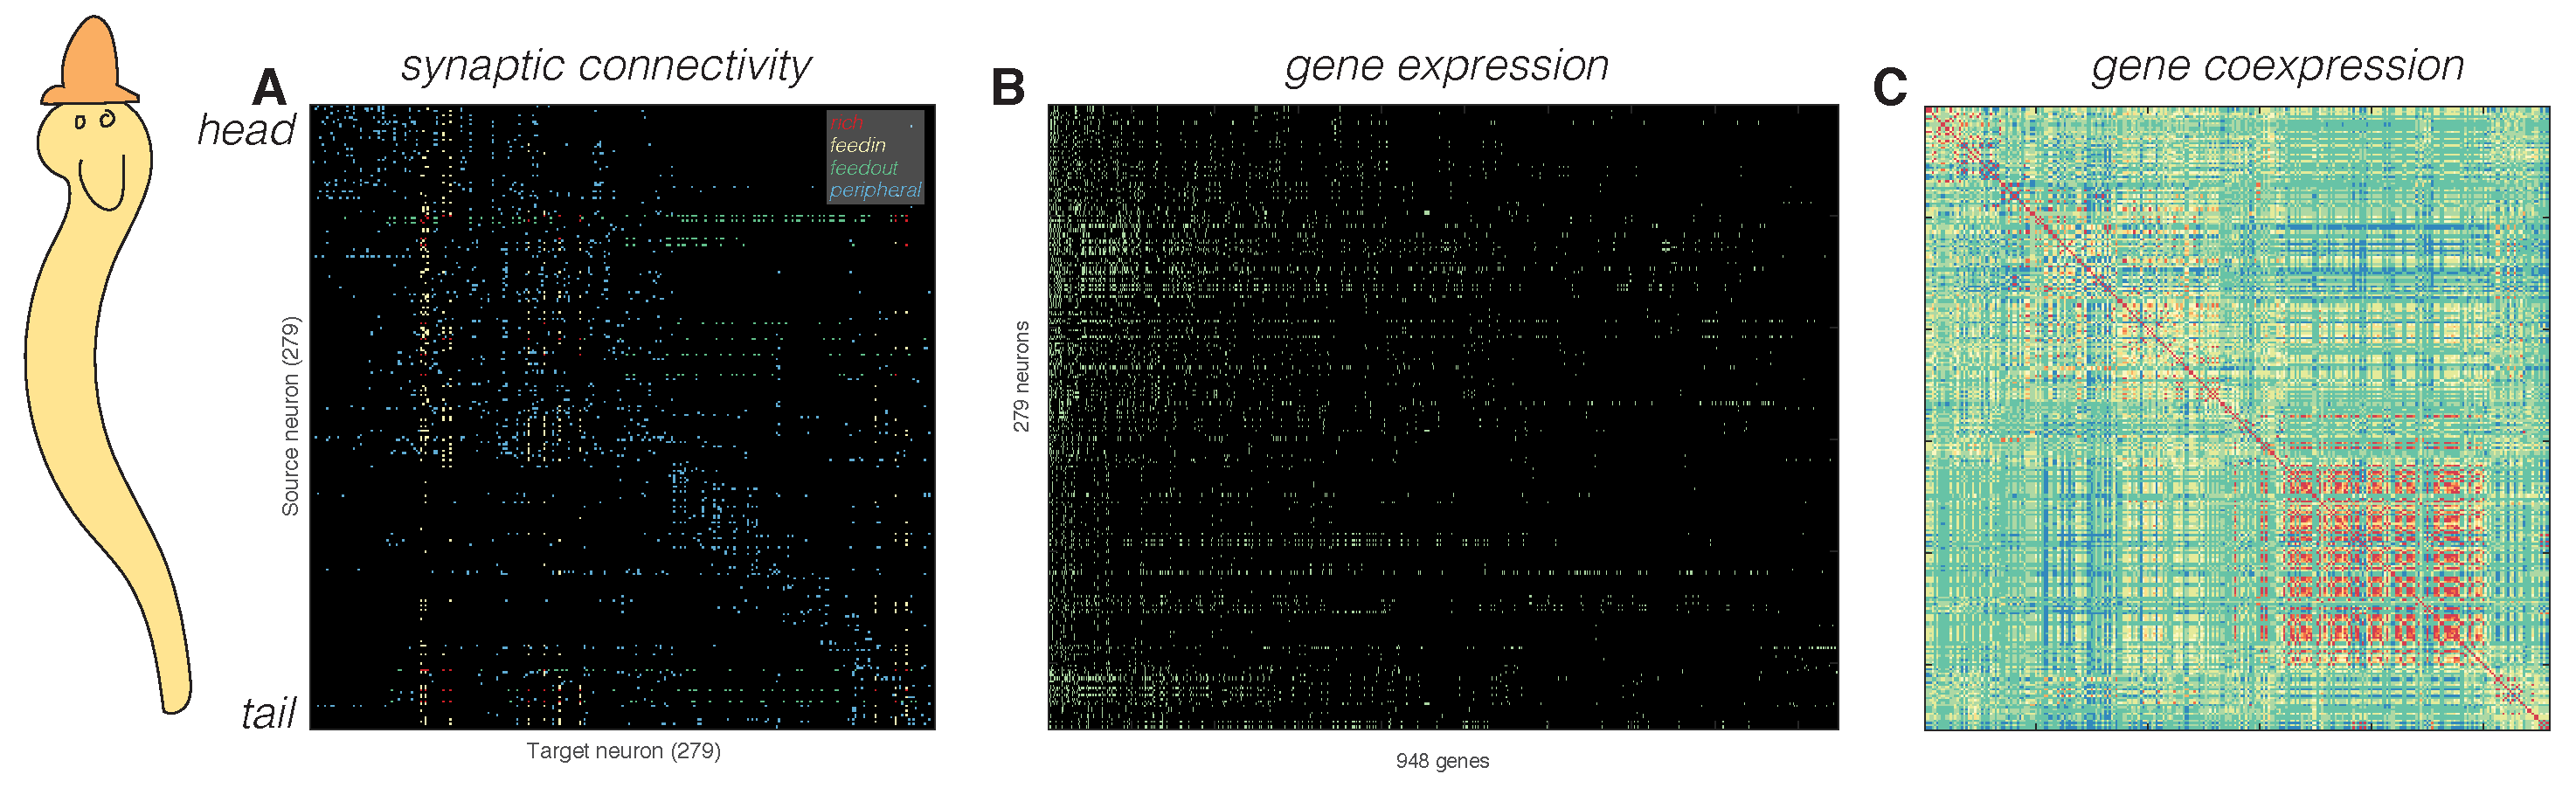
\includegraphics[width=1\textwidth]{schematic.pdf}
 \caption{\textbf{Schematic data representation}
 \textbf{A} Binary synaptic connectivity between all pairs of neurons, colored according to type: rich, feeder, and peripheral.
  \textbf{B} Gene expression across the 948 genes that are expressed in at least one neuron.
 \textbf{C} Gene coexpression matrix.
[[TODO: I think it would be nice to put neuronal metadata on the edge]]
Neurons have been ordered by their position, from head (upper) to tail (lower).
}
\label{fig:SchematicRepresentation}
\end{figure}


%%
\subsection*{Hub connectivity in the C. elegans connectome}
%% INTRODUCE RICH CLUB  hene and focus on the difference between rich/feeder/peripheral links below

% \paragraph{Rich club organization of the connectome}

% <<hubs>>
First, we analyze the topological properties of the C. elegans connectome, represented here as a directed, binary connectivity matrix of the 1961 chemical synapses between 279 non-pharingeal neurons \cite{Varshney2011}, focusing particularly on hub connectivity.
The degree distribution of the C. elegans chemical connectome is shown in Fig.~\ref{fig:topology_rich}A, where neurons have been distinguish according to type: 68 sensory neurons, 85 interneurons, 108 motor neurons, and 18 neurons that have multiple annotations (annotations from WormBase (\url{ftp://ftp.wormbase.org/pub/wormbase/releases/WS256/ONTOLOGY/anatomy_association.WS256.wb}, release WS256, date 6th Feb 2017 AA: already referenced WormBase in the beginning). 
Consistent with previous work [[]], we see a positively-skewed degree distribution containing an extended tail of high-degree hubs, the majority of which are interneurons [[characterized in previous work as control INs]].

% ------------------------------------------------------------------------------
% <<TopologyFigures.m>>
% ------------------------------------------------------------------------------
\begin{figure}[h]
   \centering
    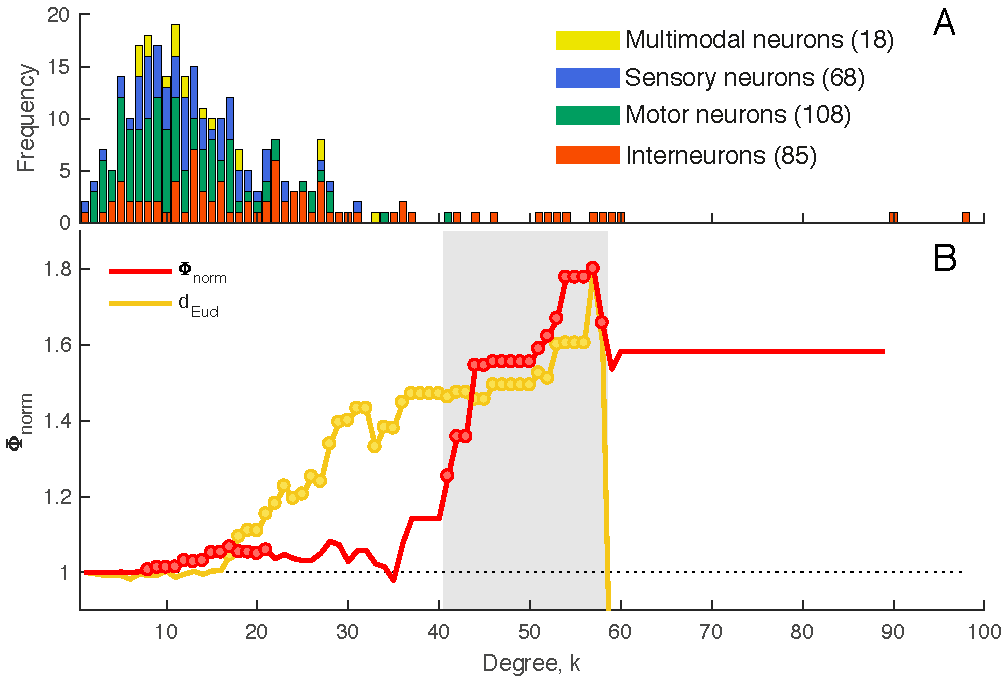
\includegraphics[width=0.9\textwidth]{topology_rich.pdf}
    % 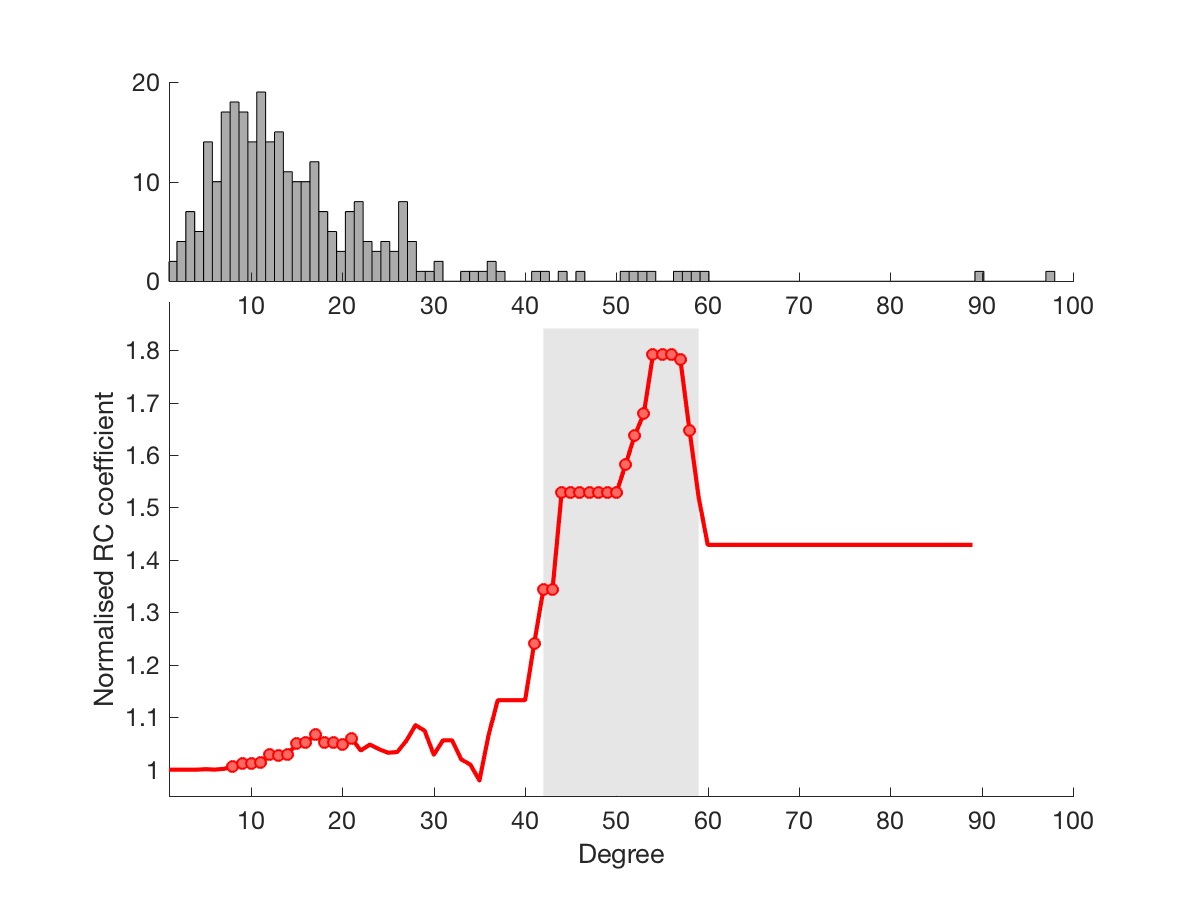
\includegraphics[width=0.7\textwidth]{RCcurve.eps}
 \caption{\textbf{Rich-club organization of the connectome}.
% A: Topological rich-club. B: Mixed rich-club. C: Weighted rich-club.
\textbf{A} Degree distribution of the binary chemical connectome, where neurons are labeled according to four categories:
(i) interneuron (85 neurons, orange),
(ii) sensory (68 neurons, blue),
(iii) motor (108 neurons, green), or
(iv) multiple assignments (18 neurons, yellow).
An extended tail of high-degree neurons can be seen, which are mostly interneurons.
\textbf{B}
Normalized rich club coefficient, $\Phi_\mathrm{norm}$ (red), as a function of the degree, $k$, at which hubs are defined (as neurons with degree $>k$).
Also shown is the mean Euclidean separation distance (yellow) between connected hub regions (across degree thresholds, $k$).
$\Phi_\mathrm{norm} > 1$ indicates that hubs are more densely interconnected among each other than expected by chance, with red circles indicate values of $\Phi_\mathrm{norm}$ that are significantly higher than an ensemble of 1\,000 degree-matched null networks ($P < 0.05$).
Yellow circles indicate where the Euclidean distance between connected pairs of hubs is significantly greater than the Euclidean distance for all other pairs of connected regions (Welch's $t$-test, $P < 0.05$).
[[TODO: maybe avoid yellow to mean two different things within the same plot... Could either change distance or the multiple assignment color]]
}
 \label{fig:topology_rich}
 \end{figure}
% ------------------------------------------------------------------------------

% <<rich-club organization>>
We quantified the extend to which hubs are densely interconnected by computing the normalized rich-club coefficient, $\Phi_\mathrm{norm}$, with $\Phi_\mathrm{norm} > 1$ indicating rich-club organization of the network.
The variation in $\Phi_\mathrm{norm}$ across a range of thresholds, $k$ (at which hubs are defined, as neurons with degree $>k$), is shown in Fig.~\ref{fig:topology_rich}B, with red circles indicating a significant increase in link density among hubs relatively to 1\,000 degree-preserving nulls (permutation test, $P < 0.05$) [[check whether randmio\_dir only preserves degree]].
The plot reveals rich-club organization at the upper tail of the degree distribution, particularly for thresholds $41 < k < 58$, referred to here as the `topological rich-club regime', shaded gray in Fig.\ref{fig:topology_rich}B.
% This indicates that when nodes are defined as hubs (degree $>\textit{k}$) in this range, they are more densely interconnected than expected by chance.
Most of the analyses performed here compare variation as a function of the hub threshold, $k$, but for analyses requiring a fixed hub definition, we define hubs as the 13 neurons with $k > 41$ [[TODO: compare to Towlson]].
% Rich club in the chemical synapse network consists of 13 high degree neurons with degree $42 \leq k \leq 98$.

[[maybe include a list with degrees and definitions in SUPP (like in Towlson's paper?). Are our hubs similar of different? Why? SIMILAR, but different degree as we use a slightly different connectome).]]

% <<distance, geometric effects>>
Recent work has shown that many aspects of connectome organization can be partially accounted for by geometric effects, that treat the connectome not just as an abstracted graph topology, but as a spatially-embedded object \cite{Henderson:2014fg, Roberts2016, Horvat:2016ia}.
In Fig.~\ref{fig:topology_rich}B, we plot the mean distance between all pairs of connected hubs at each degree threshold, $k$, finding an increase in mean hub-hub connection distance with $k$, through to the extent of the topological rich-club regime.
This increase can be attributed to a relative increase in connections between the head and tail in hub-hub connections relative to other connection types [[TODO: should we show evidence in the supps?]].
Despite an increase in hub-hub connection density across longer distances, connection probability decreases with distance in C. elegans (see Fig.~\ref{fig:S_distDep}A, particularly for head-head and tail-tail connections, up to $\approx 0.2$\,mm, and body-body connections up to $\approx 0.4$\,mm, and head-tail and tail-head connections, from $\approx 1.0-1.2$\,mm), mirroring recent results in mouse \cite{Goulas:2016hr, Fulcher:2016ck}, and other rodents and primates \cite{Horvat:2016ia}.
Taken together, our results demonstrate that hub-hub connections in C. elegans are dense, and extend over significantly longer distances than other types of connections in the synaptic connectome, consistent with the idea of the rich club as a costly but central backbone for neuronal communication \cite{vandenHeuvel:2012kh}.


% In connectomes across species and scales, degree is distributed unequally, with a small number of highly connected brain regions, known as hubs \cite{Sporns:2007ea}, that are themselves more densely connected between themselves, forming a so-called `rich club' \cite{deReus:2013cy, ZamoraLopez:2010hy, Shih:2015cu, vandenHeuvel:2012kh, vandenHeuvel:2011he}.
% The same is true in the C. elegans neuronal nervous system, analyzed in the past as an undirected binary connectome including both chemical and electrical synapses \cite{Towlson:2013gf}, which exhibits highly connected, and densely interconnected hub neurons.

%%
\subsection*{Coexpression and connectivity}

% ---connectivity/coexpression---
Having characterized the topological and geometric properties of connectivity, in particular the rich-club organization of hub neurons, we next investigate how connectivity properties relate to patterns of neuronal gene expression.
Being a pairwise analysis, we compare pairwise synaptic connectivity to pairwise similarity in gene expression (using a binary Pearson correlation measure, $r_\phi$, to define gene coexpression, and excluding coexpression values between homologous left/right neuron pairs, see Methods).

We first investigated whether gene coexpression relates to synaptic connectivity by comparing the distribution of $r_\phi$ computed for all connected pairs of neurons, and for all unconnected pairs of neurons, as shown in Fig.~\ref{fig:coExp}A.
We find that connected pairs of neurons have more similar expression profiles than unconnected pairs (Wilcoxon rank-sum test, $P < 10^{-50}$).
Using directed connectivity information to split connections into unidirectional ($X \rightarrow Y$) and reciprocal ($X \leftrightarrow Y$) subtypes, we found no difference in coexpression as a function of connection reciprocity, but both groups showed an increase in coexpression relative to unconnected pairs of neurons (see Fig.~\ref{fig:S3_Fig} ).


% ------------------------------------------------------------------------------
% <<coexpConnUncon.m>>
% <<RichClubMedian.m>>
% ------------------------------------------------------------------------------
 \begin{figure}[h]
 \centering
    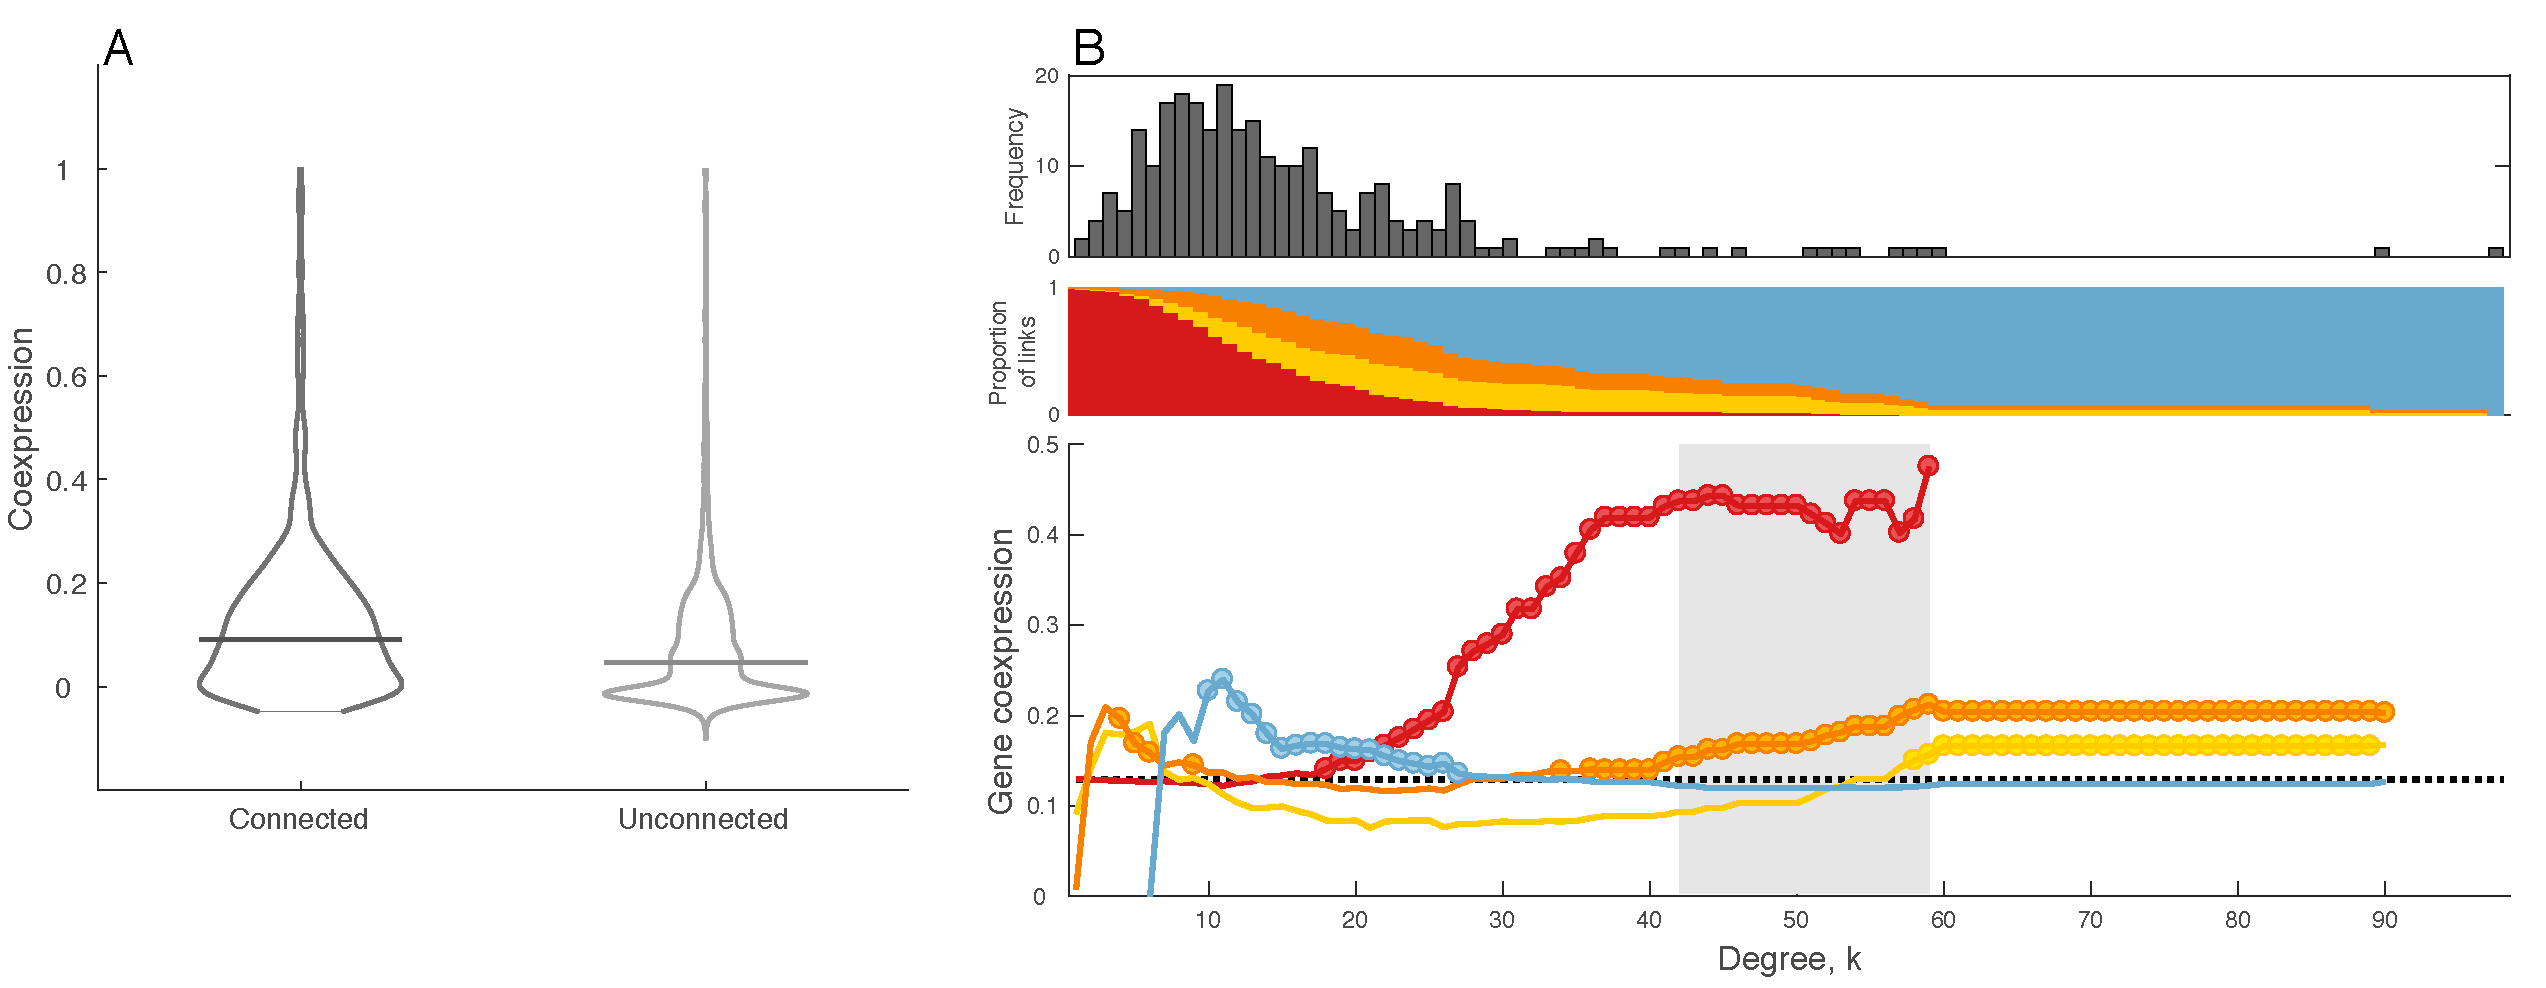
\includegraphics[width=1\textwidth]{MeanCoexpression2.pdf}
 \caption{{\bf Gene coexpression varies as a function of connectivity, and as a function of connection type, with connections involving hubs being most similar.}
\textbf{A} Distribution of transcriptional similarity between connected ([[XX]] pairs) and unconnected ([[XX]] pairs) pairs of neurons as a violin plot, with the mean of each distribution shown as a horizontal line.
Coexpression, $r_\phi$ is increased in connected pairs of neurons ($P < 10^{-50}$, Wilcoxon rank sum test).
\textbf{B}
\emph{Top}: Degree distribution.
\emph{Middle}: proportion of connections that are `rich' (hub$\rightarrow$hub, red), `feed-in' (nonhub$\rightarrow$hub, yellow), `feed-out' (hub$\rightarrow$nonhub, orange), and `peripheral' (nonhub$\rightarrow$nonhub, blue) as a function of the degree threshold, $k$, used to define hubs.
Note that at high $k$, most neurons are labeled as nonhubs, and hence the vast majority of connections are `peripheral'.
\emph{Lower}: Median Pearson gene coexpression, $r_\phi$, for each connection type as a function of $k$.
The median coexpression across all network links shown as a dotted black line; the topological rich-club regime (determined from the network topology, cf. Fig.~\ref{fig:topology_rich}) is shaded gray.
Circles indicate a statistically significant increase in gene coexpression in a given link type relative to the rest of the network (Wilcoxon rank sum test; $P < 0.05$).
[[TODO: A: add $r_\phi$ to ylabel.).
B: Remove box from degree distribution, Change y-label to `Median gene coexpression', fonts are small, and inconsistent sizes between subplots.
I think we should crop the curves when there are fewer than X connections remaining -- in this case it's a bit ridiculous to show that constant feed-out/feed-in/peripheral coexpression when there are only two neurons
left as hubs]]}
 \label{fig:coExp}
\end{figure}
% ------------------------------------------------------------------------------

% ---HUB coexpression---
Having established an increase in gene coexpression in connected pairs of brain regions (relative to unconnected pairs), we next investigated whether coexpression varied between different types of connections, focusing particularly on the role of densely interconnected hub nodes characterized above.
Given the importance of hub neurons across species [[Ref]], and previous results in the mesoscale mouse connectome \cite{Fulcher:2016ck}, we expect increased coexpression in connections involving hubs.
To investigate this effect, we first labeled each neuron as either a hub (nodes with degree $> k$) or a nonhub (degree $\leq k$), for a given hub threshold, $k$, and then labeled each connection as either `rich' (hub $\rightarrow$ hub), `feed-in' (nonhub $\rightarrow$ hub), `feed-out' (hub $\rightarrow$ nonhub), or `peripheral' (nonhub $\rightarrow$ nonhub).
[[TODO: Establish whether we're computing pairs of hubs (e.g., for `rich'), or for every connection between any pair of hubs -- i.e., do reciprocal connections contribute twice to the distribution at each $k$?]]
The median coexpression for each of these four connection types described above is plotted in Fig.~\ref{fig:coExp}B, with circles indicating statistically significant increases of a given connection type (relative to all other connections) [[TODO: Why are we suddenly doing medians? subplot A is mean, right? Is median a better summary of the distribution than mean? Depending on distributions, the mean MAY raise fewer flags if results are similar using mean. ALL plots now are done using mean. Results in general are the same. I thought to use median instead of the mean because of non-normal distributions]].
We see that gene coexpression in rich connections increases with degree, reaching a plateau through the topological rich-club regime where hubs are densely interconnected (shaded in Fig.~\ref{fig:coExp}B).
Interestingly, we see a split between feed-in and feed-out connections, with feed-out connections showing increased gene coexpression through the topological rich-club regime, while feed-in and peripheral connections show the lowest levels of coexpression.
% We observed a difference in gene coexpression between feed-in and feed-out links, where feed-out links manifested increased coexpression for a broad range of degrees while feed-in links showed only a slight increase for very high hub thresholds.

These results, using partial binary expression estimates in 948 genes in a neuronal connectome, are broadly consistent with results in 213 regions of the mesoscale mouse connectome with over 17\,000 genes, in which we see an increase in coexpression in connected pairs of neurons, and the greatest coexpression amongst hub-hub connections and the lowest coexpression amongst nonhub-nonhub connections.
In contrast to the mouse connectome, however, in which hubs were distributed across a broad range of anatomical divisions, hubs in C. elegans are [[mostly. There is one motor neuron in there, right?AA: with threshold k>41, all interneurons]] interneurons \cite{Towlson:2013gf} (cf. Fig.~\ref{fig:topology_rich}A).
To determine the specificity of the effect between different neuron types, we split our coexpression analysis into connections involving: (i) interneurons, (ii) sensory neurons, and (iii) motor neurons, computing the median coexpression within each class of connections as a function of the degree of the given neuron type [[TODO: is this true? It's kind of complicated to explain -- is it right that for a given k threshold we include, say, sensory neurons of degree greater than $k$ and their connections to all other neurons in the `sensory' category? Or do we include all neurons with degree $>k$ and compute the median of those connections that involve both the high-degree neurons AND neurons of the given class? This would be another choice. Perhaps it's the latter that's plotted?YES: now we include connections for 'sensory' deg>k to any other other neurons with degree >k - my code is is really complicated - probably there is much easier way to do the same]], as shown in Fig.~\ref{fig:interneuron_dep}A.
Note that the three categories are not mutually exclusive; for example, the `interneuron' class includes connections between any interneuron and any other neuron.
We find that connections involving interneurons are unique in their increasing [[average]][[median? See comments above about whether to use mean throughout... Need to inspect the distributions to motivate the right choice]] coexpression with increasing degree, $k$.
Connections involving motor neurons, and connections involving sensory neurons, do not show any clear increase with degree.

\begin{figure}[h]
\centering
   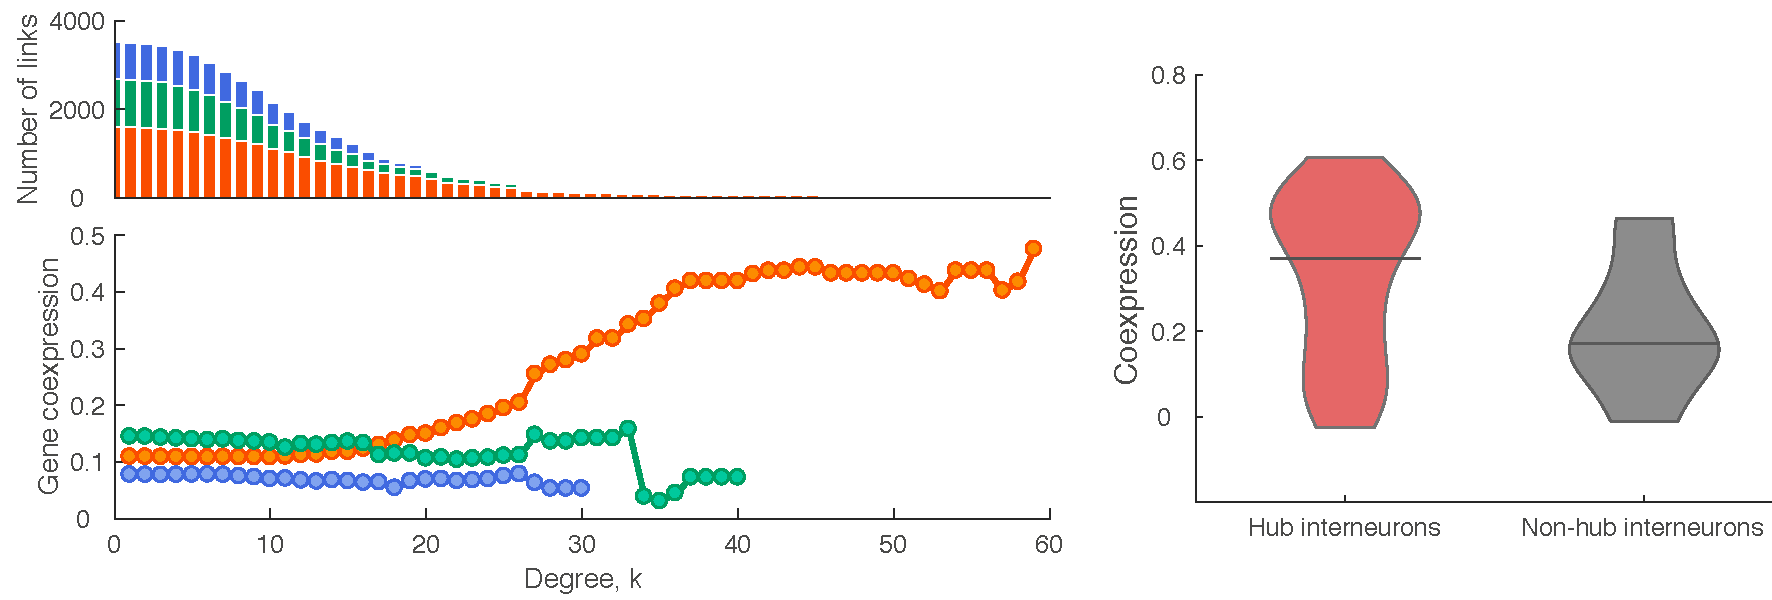
\includegraphics[width=1\textwidth]{TypeDegree.pdf}
 \caption{
\textbf{The increase in coexpression with degree is specific to high-degree interneurons, and hub interneurons have higher coexpression than nonhub interneurons.}
\textbf{A} \emph{Upper}: The number of connections involving interneurons (orange), sensory neurons (green), and motor neurons (blue) across degree threshold, $k$ [[TODO: Aurina, is it correct that sensory is green and motor is blue?AA: NO - motor are green, sensory blue (I changed RC degree distribution colors in the PlotRichClub.m script accordingly)]].
\emph{Lower}: Average gene coexpression as a function of degree for connections involving different types of neurons.
\textbf{B} Coexpression distributions for all pairs of hub interneurons (red) and all pairs of non-hub interneurons (gray).
[[TODO: Did we exclude multimodal neurons from this analysis?? Can we do a statistical comparison between these distributions and add something here on that?]]
[[TODO: A: the vertical axis in lower subplot should state `median gene coexpression']]
[[TODO: Both coexpression axes should be the same `Gene coexpression, $r_\phi$']]
 \label{fig:interneuron_dep}
}
\end{figure}

Given the distinction of interneurons in driving the gene coexpression relationship with degree, $k$, we next verified whether hubs showed a unique transcriptional signature among this neuronal subtype.
We compared gene coexpression between all pairs of hub interneurons [[TODO: what $k$ threshold?]] and between all pairs of nonhub interneurons (AVFL, AVFR, AVHL, AVHR, AVKL, AVKR, AVJL, AVJR) [[TODO: what does this list represent? Not clear from the sentence structure]], as shown in Fig.~\ref{fig:interneuron_dep}B.
% that share similar anatomical properties in order to ensure that increase in coexpression for rich links is not determined by the fact that the majority of hub neurons belong to the same anatomical neuron type (???HOW TO CALL COMMAND INTERNEURONS???).
% In order to compare transcriptional similarity between all pairs of neurons we ignore the existence (or absence) of connections between these neurons,
Pairs of hub interneurons display significantly higher gene coexpression than pairs of nonhub interneurons ([[TODO: statistical test, p-value, etc.]]).
Thus, the increase in coexpression amongst hub interneurons is not simply due to most hubs being interneurons;  even amongst interneurons, [[TODO: isn't this obvious from plot A? It's very similar -- at high degree, we're only looking at hub interneuron pairs, which are more similar than others. Not sure B adds much -- we could just quantify the difference at a given $k$ threshold to put a statistic to it...?AA: it adds inf, besause we're comparing hubs to interneurons with the same anatomical properties, not just random low degree interneurons. PLOT A says - effect driven by interneurons (other groups of neurons do not show this increase with degree), plot B says - among interneurons that are anatomically the same (hub interneurons and 8 interneurons that are not hubs), hubs have higher coexpression]].\\

\textbf{Birth time}. 
All hubs are born early in the \textit{C. elegans} development \cite{Varier2011}, therefore we next verified that the increase in coexpression between them can not be explained by the similarity in birth time. 
For this purpose, we separated neurons that are formed early (during the first 1000 min) in the development into two types, namely hubs and non-hubs, and compared coexpression within each of those groups (Fig \ref{fig:BirthTimeHubs}). 
Links between hubs show significantly increased coexpression and consequently confirm that even between the neurons that were born roughly at the same time, hubs exhibit a unique transcriptional pattern.
\begin{figure}[t]
  \centering
    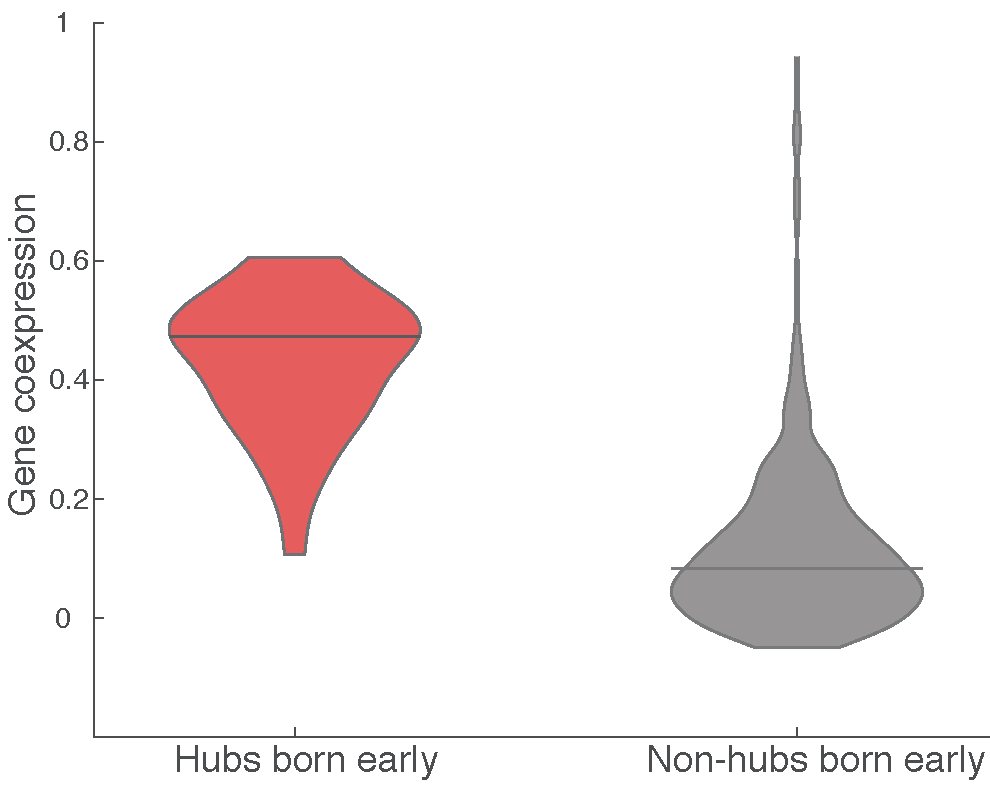
\includegraphics[width=0.5\textwidth]{BirthTimeHubs.pdf}
 \caption{\textbf{Coexpression between early born hubs and early born non-hubs. COULD DO BORN EARLY OR BORN TOGETHER} ($P < 10^{-28}$, Wilcoxon rank sum test)
}
\label{fig:BirthTimeHubs}
\end{figure}


\subsection*{Hubs and modules}
Having demonstrated an increase in coexpression with connectivity and, amongst connections, with hub connectivity, we next investigate whether other influences, namely modular organization, lineage similarity, or neurotransmitter type, could explain our results.

% \paragraph{Distance}).
% Implementing the same methods as previously used in gene coexpression analysis at each degree threshold for each link type (rich, feeder, peripheral) we calculated the mean connection distance.
% Connection distance increased with increasing degree for both rich and feeder links while peripheral connections demonstrated no increase through the whole range of thresholds (Fig.~\ref{Distance}).
% Given this result, it is safe to say that increased coexpression for hub-related links is not determined by lower connection distance between them as the contrary is shown to be true.

%\begin{figure}[!h]
%\centering
 %   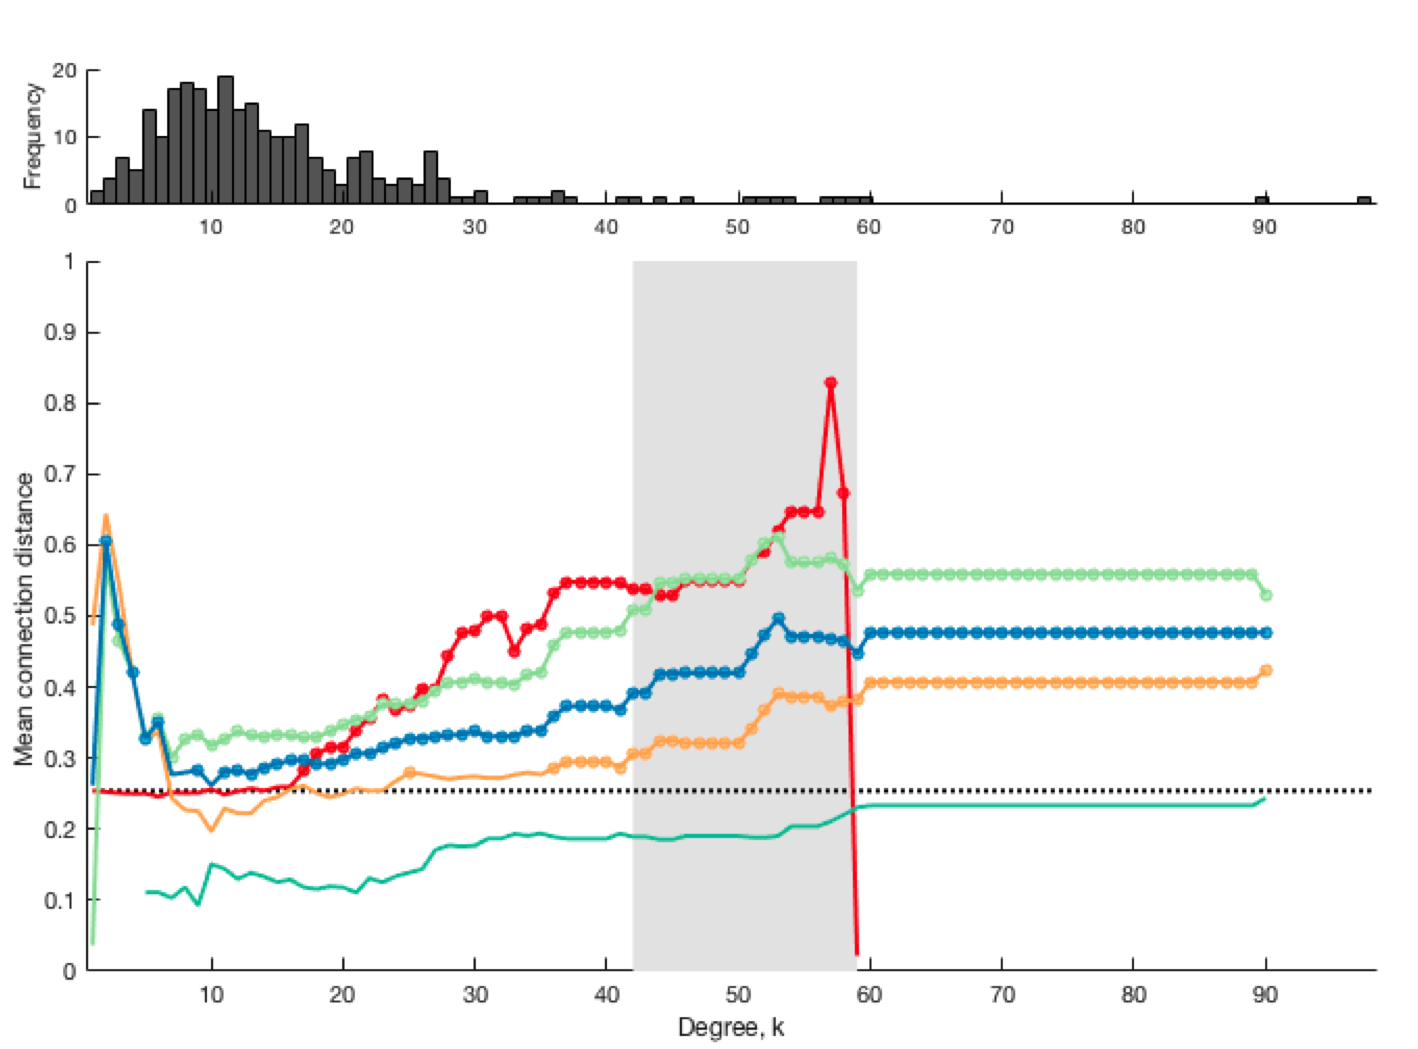
\includegraphics[width=0.7\textwidth]{distance_k}
 %\caption{{\bf Connection distance as a function of degree}}
 %\label{Distance}
 %\end{figure}

The nervous system of \emph{C. elegans} is modular [\cite{Kim2014a,Bassett2010a,Pavlovic2014  }], containing densely connected groups of neurons that are relatively sparsely connected to other neurons.
To test the possibility that gene expression differences of modules (e.g., between intra-modular and inter-modular connections) might drive the increased gene coexpression of hubs, we used the Louvain community detection algorithm (see \textit{Methods}) to extract modules from the binary C. elegans synaptic connectome, shown in Fig.~\ref{fig:modules}A.
In this analysis, hubs are mostly concentrated in a single module (purple in Fig.~\ref{fig:modules}), but are also distributed across three other modules.
% The algorithm detects three comparably sized modules (M1-M3), each containing diverse neuron types, as well as a smaller fourth module (M4), which contains 13 motor neurons.
% Of the 13 hubs with $k \geq 42$, the majority (11) were assigned to M3, which spanned the length of the worm body, as pictured in Fig.~\ref{fig:modules}.
The module most concentrated in hubs is diverse, containing neurons across the head, tail, and body and contains sensory, motor, and interneurons (see labels on Fig.~\ref{fig:modules}A).
This module is particularly concentrated in motor neurons, consistent with evidence that control interneurons are directly responsible for forward and backward locomotion (command interneurons).
% 10 out of 11 hub neurons in this module are directly responsible for
% The main goal of this analysis was to compare coexpression within and between modules in order to examine if neurons assigned to the same module are more genetically similar than neurons in other modules.
Gene coexpression, $r_\phi$, was in fact slightly lower in intra-modular connections relative to inter-modular connections (Fig.~\ref{fig:modules}B, $p = 0.045$, Welch's t-test), but intra-modular connections between hubs were increased relative to other intra-modular connections (Fig.~\ref{fig:modules}C, $p = 1.3\times 10^{-10}$).
We also computed an empirical null distribution for the mean coexpression for hub-hub links, given they span 34 intra-modular links and 32 inter-modular links; 1\,000 samples from such an intra/intermodular link distribution gives a null $r_\phi$ of $0.15 \pm 0.02$, compared to the observed value of $0.51$ ($p < 10^{-16}$).
% Coexpression within modules did not exceed coexpression between modules, demonstrating that neurons that belong to the same module do not share any particular genetic similarity.
The increased coexpression in connected pairs of hubs in C. elegans can therefore not be attributed to the modular organization of the connectome.
% despite most hubs being assigned to the same module.
% [[NOTE: maybe not worth characterizing modules, just say: coexpression within modules is not higher than coexpression between modules on one sentence and distributions? When hub neurons are excluded, M2 and M3 coexpression is higher than M1, but no difference between M2 and M3]])

% ------------------------------------------------------------------------------
% <<plot_modules.m>>
% ------------------------------------------------------------------------------
\begin{figure}[!h]
\centering
    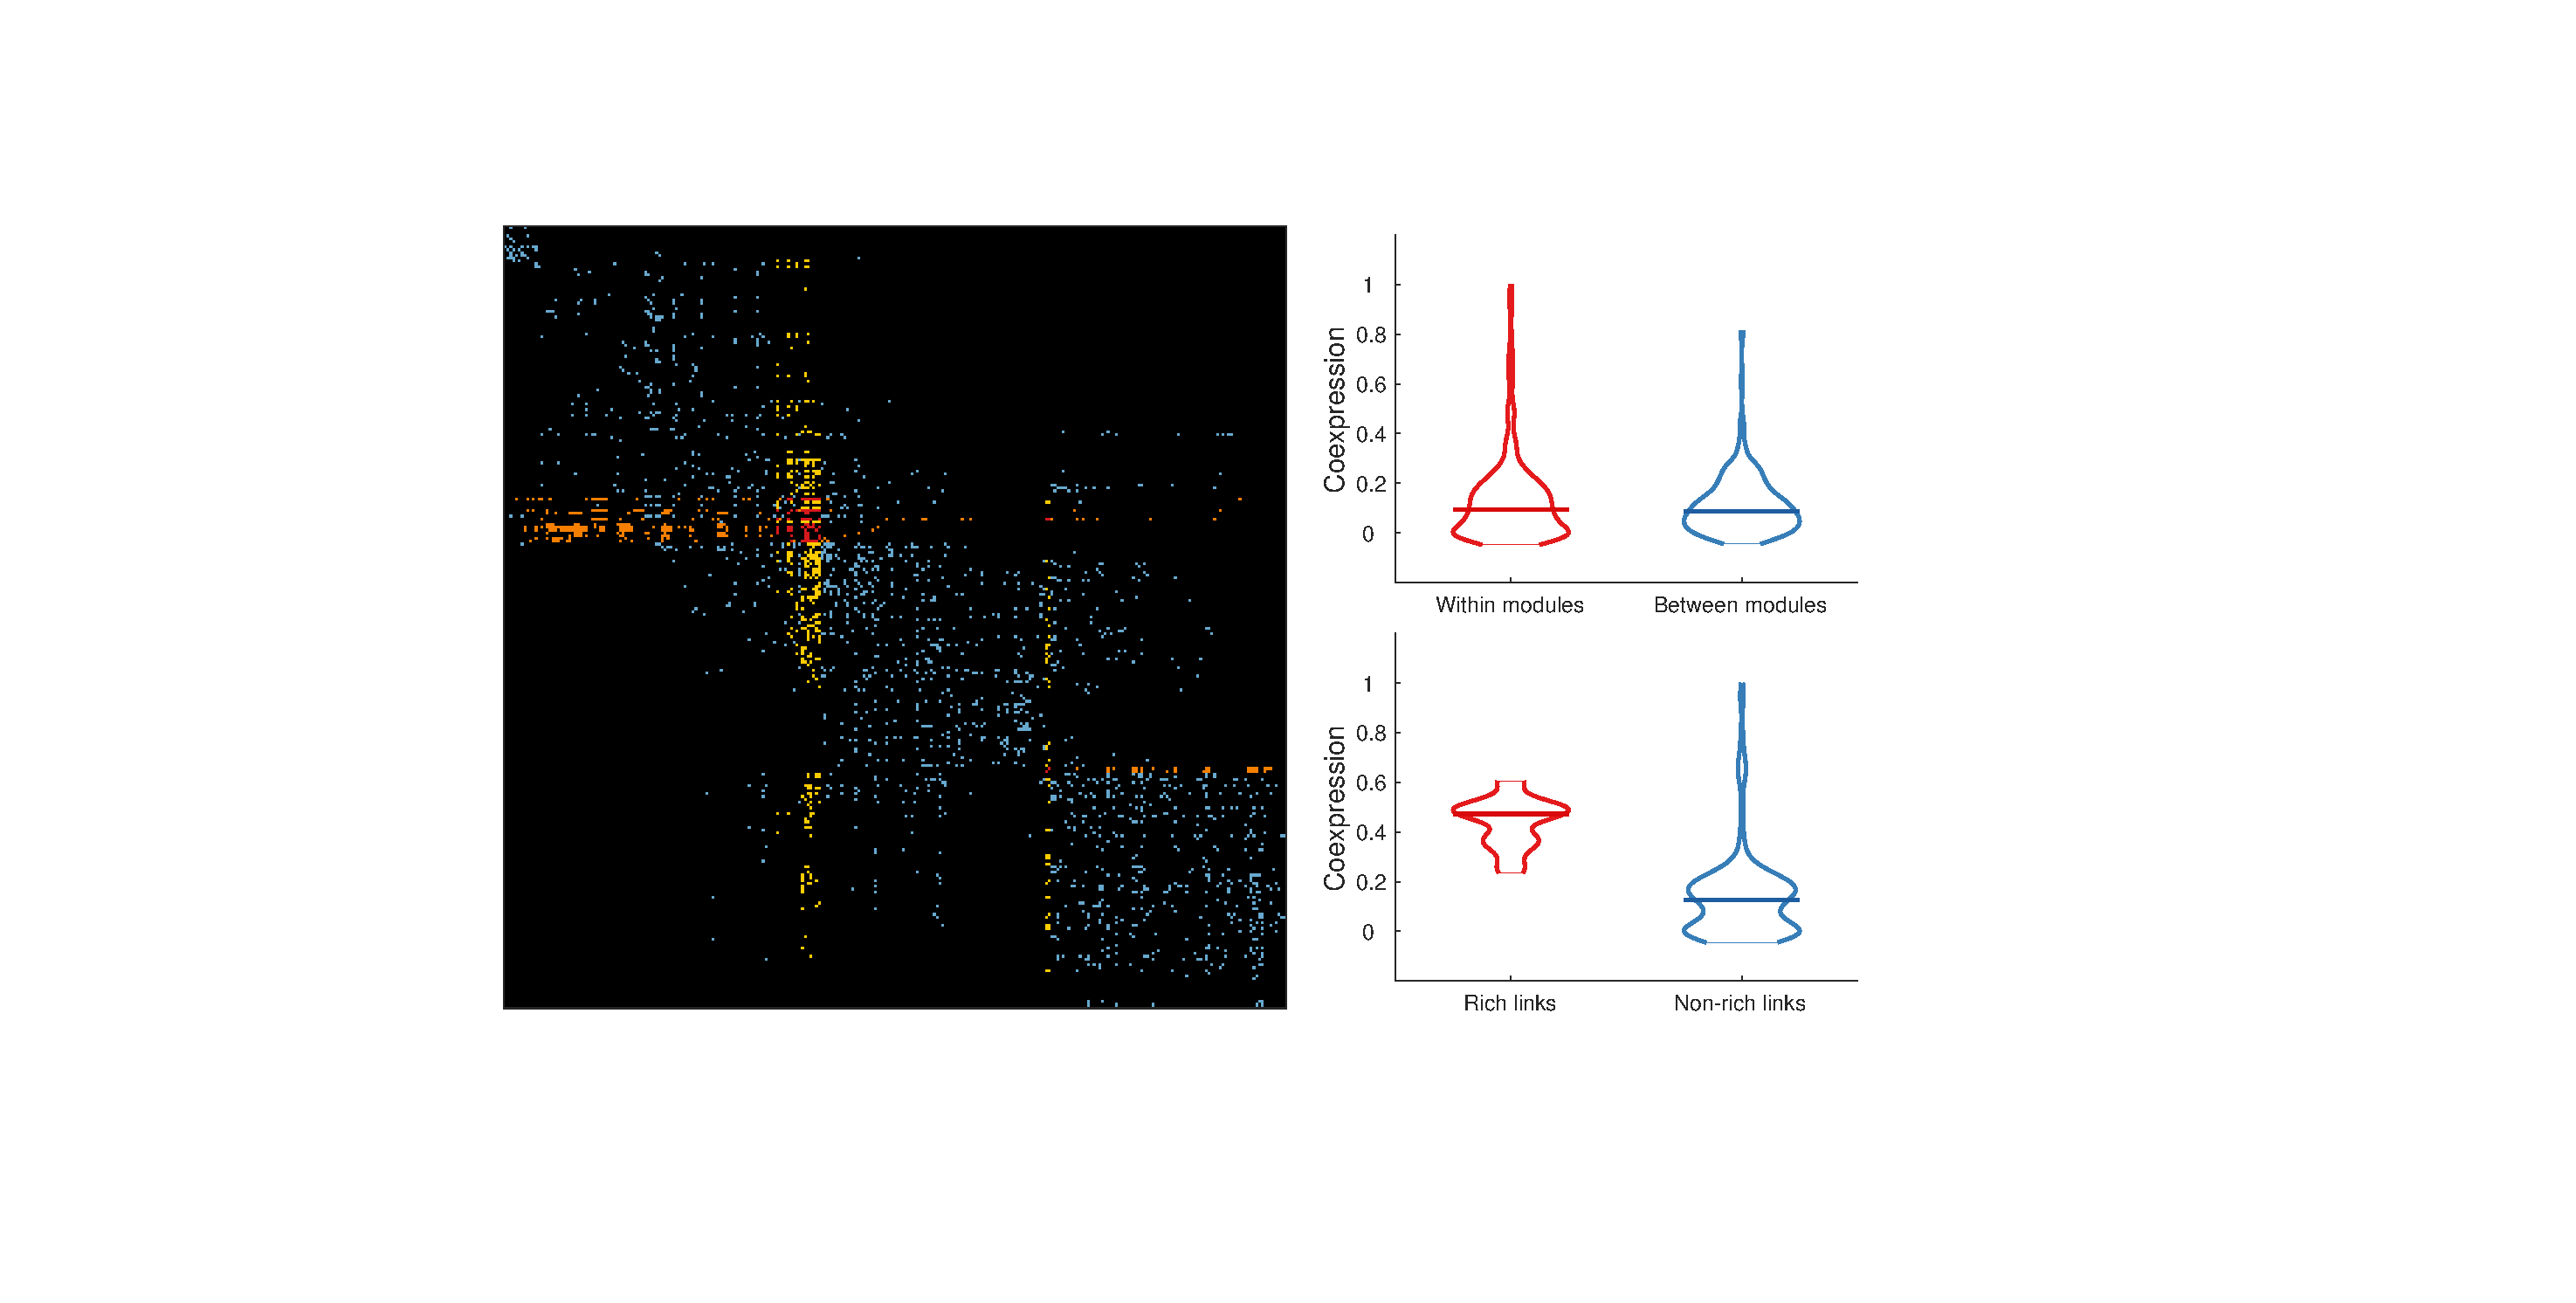
\includegraphics[width=1.2\textwidth]{Modules.eps}
 \caption{
 \textbf{Increased coexpression of hub neurons are not driven by their module membership}
%\textbf{A: Connection distance}
%Top: Degree distribution.
%Bottom: Median lineage distance for rich, feeder, and peripheral connections as a function of \textit{k}, with the %median across all network links shown as a dashed black line and the topological rich club regime shaded grey.
%Circles indicate a statistically significant change in lineage distance in a given link type relative to the rest %of the network (Wilcoxon rank sum test; $P < 0.05$). \\
\textbf{A} Connectome organized by module (white squares), with all connections labeled by type: rich (red), feed-in (yellow), feed-out (orange), and peripheral (blue).
Neuron indicators are shown to the left, including module assignment, neuron type (interneuron, orange; motor neuron, blue; sensory neuron, green; multimodal, yellow), hub indicator (red for hubs), position along the body, from head (white) to tail (black), and neuron type: head (yellow), body (orange), tail (red).
\textbf{B} Distributions of gene coexpression, $r_\phi$, for intra-modular connections (black) and inter-modular connections (gray), shown as violin plots with the mean shown as a horizontal bar.
The number of connections of each type is shown in parentheses.
\textbf{C} Violin plots of the distributions of $r_\phi$ for intra-modular hub-hub connections (black) compared to other intra-modular connections (gray).
%Composition of each module according to neuron type.
%Modular organisation of the connectome.
%Coexpression distributions within and between modules.
%\textbf{C: Lineage distance}
%Top: Degree distribution. Bottom: Mean lineage distance for rich, feeder, and peripheral connections as a function %of \textit{k}, with the median across all network links shown as a dashed black line and the topological rich club regime shaded grey.
%Circles indicate a statistically significant change in lineage distance in a given link type relative to the rest of the network (one-sided Welch’s t-test; $P < 0.05$) \\
%\textbf{D: Coexpression for different types of neurons. }
%Top: Median gene coexpression as a function of degree for connections involving different types of neurons.
%Bottom: The number of connections in each category for a range of degrees.
%Coexpression distributions for hub and non-hub interneurons. \\
[[TODO: Label modules (large), but also neuron types, neurotransmitters, etc. along the rows]]
}
 \label{fig:modules}
\end{figure}


Lineage distance between pairs of neurons presents another source of information about the genetic makeup of the \textit{C. elegans} nervous system.
It has been shown in \textit{C. elegans} that cells with identical fates can be formed by different gene regulatory pathways \citep{Liu2009}, however, to the best of knowledge, no lineage distance analysis was done in relation to the network properties of the \textit{C. elegans} connectome.
Implementing an analogous strategy as in our previous analysis of gene coexpression, we show that lineage distance between pairs of neurons increases with degree for feeder links while no significant change is observed for rich links (Fig. \ref{Lineage}).
This finding suggests that the difference in lineage distance between hub and non-hub neurons increases with degree, therefore in a way confirming the relevance of this classification.
Contrary, peripheral links manifest stably lower lineage distance through the range of degree thresholds wit (Fig. \ref{Lineage}).
In addition, this shows that increase in gene coexpression with degree for rich links can not be attributed to their similarity in lineage.

Is it possible to say that connections within ACh are more similar when they involve hubs?

\subsection*{Functional enrichment}

%% comment on enrichment analysis. No write up can be done before deciding on options.

To investigate which functional groups of genes contributed to the difference in transcriptional coupling between connected and unconnected neurons, we used a method of assigning each gene coexpression contribution (GCC) score that quantifies the contribution of each gene to the overall coexpression between neuron pairs (see Methods).  \\

The majority of the significant ($P < 0.05$) GO categories are related to neuronal connectivity and communication, as listed in Table~\ref{table1} (1st column: GO category).
These findings are in line with our expectations as they confirm that genes that are more likely to be expressed in a pair of connected neurons are in fact related to neuronal connectivity and communication.\\

To investigate which functional groups of genes contributed to the increased coexpression for links involving hubs (rich and feeder) we again we used a method of scoring genes according to their contribution towards increased coexpression (see Methods).

Enrichment analysis show that the majority of the significant ($P < 0.05$) GO categories are related to glutamate signaling, neuronal connectivity and communication.
It is line with the previous analysis where same GO categories were shown to be significant in differentiating connected from unconnected neurons.

%% Combined enrichment table
\begin{table}[t]
\begin{adjustwidth}{-2.25in}{0in} % Comment out/remove adjustwidth environment if table fits in text column.
\centering
\caption{
{\bf Enrichment.}}
\begin{tabular}{ |c|c|c| }
\thickhline
%{\bf Connected} & {} & {\bf Rich and feeder}\\ \thickhline
GO category  		& Connected \textit{vs} unconnected: $P$-value  	& Rich and feeder \textit{vs} peripheral      \\ \thickhline
glutamate receptor signaling pathway      	& $10^{-7}$      		&  $10^{-5}$\\ \hline
ionitropic glutamate receptor signaling     & $10^{-7}$      		&  $10^{-5}$ \\ \hline
synaptic transmission, glutamatergic      	& $10^{-7}$     			&  $10^{-5}$ \\ \hline
neuron-neuron synaptic transmission          & $10^{-5}$     			&  0.00031\\ \hline
chemical synaptic transmission               & 0.00057      			&  $10^{-5}$\\ \hline
anterograde trans-synaptic signaling      	& 0.00057      			&  $10^{-5}$\\ \hline
synaptic signaling                          & 0.00057      			&  $10^{-5}$\\ \hline
trans-synaptic signaling                    & 0.00057      			&  $10^{-5}$ \\ \hline
cell-cell signaling                         &      -           		&  0.00086 \\ \hline
cell surface receptor signaling pathway     &       -          		&  0.00107 \\ \hline
\end{tabular}
\begin{flushleft} Table notes what GO categories were overrepresented in driving the difference between different types of links.
\end{flushleft}
\label{table1}
\end{adjustwidth}
\end{table}

These findings are in line with our expectations as high degree neurons are highly involved in signaling and the majority of hubs while being cholinergic, receive input from sensory neurons the majority of which is glutamatergic.

[[NOTE: NOTE HERE ABOUT REDUCED LIST OF GENES IN EACH ANALYSIS (577 and 390 genes for connected and R/F respectively).]]


%\begin{figure}[h]
%\centering
 %   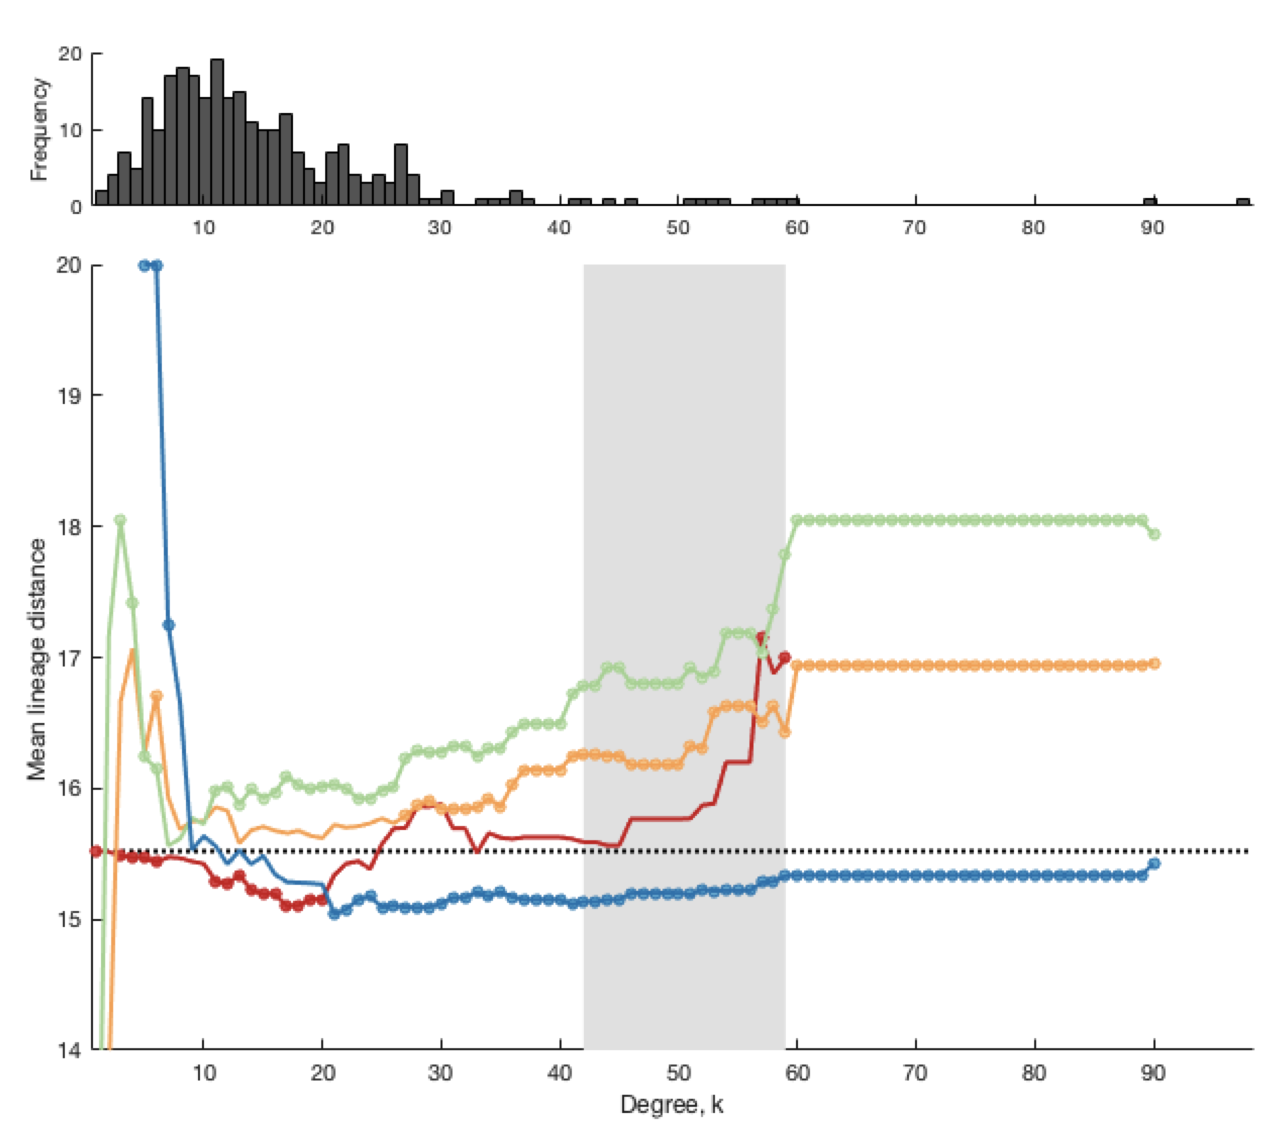
\includegraphics[width=0.7\textwidth]{LineageRFP}
 %\caption{\textbf{}
 %\label{Lineage}
 %\end{figure}


%%

% Place tables after the first paragraph in which they are cited.
% \begin{table}[!ht]
% \begin{adjustwidth}{-2.25in}{0in} % Comment out/remove adjustwidth environment if table fits in text column.
% \centering
% \caption{
% {\bf Table caption Nulla mi mi, venenatis sed ipsum varius, volutpat euismod diam.}}
% \begin{tabular}{|l+l|l|l|l|l|l|l|}
% \hline
% \multicolumn{4}{|l|}{\bf Heading1} & \multicolumn{4}{|l|}{\bf Heading2}\\ \thickhline
% $cell1 row1$ & cell2 row 1 & cell3 row 1 & cell4 row 1 & cell5 row 1 & cell6 row 1 & cell7 row 1 & cell8 row 1\\ \hline
% $cell1 row2$ & cell2 row 2 & cell3 row 2 & cell4 row 2 & cell5 row 2 & cell6 row 2 & cell7 row 2 & cell8 row 2\\ \hline
% $cell1 row3$ & cell2 row 3 & cell3 row 3 & cell4 row 3 & cell5 row 3 & cell6 row 3 & cell7 row 3 & cell8 row 3\\ \hline
% \end{tabular}
% \begin{flushleft} Table notes Phasellus venenatis, tortor nec vestibulum mattis, massa tortor interdum felis, nec pellentesque metus tortor nec nisl. Ut ornare mauris tellus, vel dapibus arcu suscipit sed.
% \end{flushleft}
% \label{table1}
% \end{adjustwidth}
% \end{table}


%PLOS does not support heading levels beyond the 3rd (no 4th level headings).

% \subsubsection*{3rd level heading}
% Text.
%
% \begin{enumerate}
%     \item{react}
%     \item{diffuse free particles}
%     \item{increment time by dt and go to 1}
% \end{enumerate}
%
%
% \subsection*{Another subsection}
%
%
% \begin{itemize}
%     \item First bulleted item.
%     \item Second bulleted item.
%     \item Third bulleted item.
% \end{itemize}

\section*{Discussion}
\begin{itemize}
    \item{First coexpression analysis in worm. Despite noisy gene expression data we get some insights into the genetic basis of connectivity on a neuronal level}
\end{itemize}

% COMPARE TO MOUSE
Compared to our previous work in the mesoscale mouse connectome \cite{Fulcher:2016ck}, the present findings in a near-fully mapped neuronal chemical connectome show similarities and differences.
Despite the incredible difference in spatial scale (from each node containing $\tilde 10^5$ neurons in mouse, to just a single neuron in worm), we found a similar basic qualitative signal of increased coexpression in connected pairs of neurons, and amongst connected pairs, the most similar expression signatures in pairs of connected hub neurons.
These overall findings were specific to connections involving interneurons, i.e., were not found in motor or sensory neurons, being driven by the relatively expression similarity of high-degree interneuron hubs, were not driven by similarity in lineage, neurotransmitter type, or modular membership, and were robust to a range of data processing choices (including connectome type, and coexpression measure).
These findings come despite sparsely annotated, binary gene expression data, with less than 5\% coverage of the full genome, with preliminary enrichment analysis indicating a role for glutamate in both connectivity and hub-connectivity.
Our results indicate that even in a highly specialized neuronal nervous system, costly hub-hub connections display a distinctive transcriptional signature that may reflect their unique functional role in the network.
Further work across different species and scales may shed light on deeper principles of how connectomes organize to facilitate efficient biological functioning.


differ significantly (being a neuronal connectome), and with so few neurons, each highly specialized, it may be hard to pick up broad expression patterns that are network topology-specific.
Quite different to the case in mouse, where regions were spread across the brain, and so effects of regional specialization of function, cytoarchitecture, gene expression were averaged, and the remaining hub-related signal could be isolated.


% LINEAGE
[[TODO: add details on lineage]] While the relationship between cell lineage and gene expression was studied in other species \citep{Cui2007, Kluger2004}.

LIMITATIONS:
\begin{itemize}
    \item Did the best we had with sparsely-annotated binary gene expression data
    \item No way of discriminating between missing data and the absence of expression
    \item only around 5 percent of genes in the genome available
    \item annotation problems: different qualifiers, loosing sensitivity/specificity if including too much or too little - need to balance
    \item Future work may have actual high-throughput RNAseq gene data for all neurons, could do this analysis properly!
    \item Would surely allow more subtle understanding of how gene expression varies with connectivity roles
\end{itemize}

\section*{Conclusion}

Conclusion text.

\section*{Acknowledgments}
Thanks to Alex Fornito, for being a big deal.

\nolinenumbers

% Either type in your references using
% \begin{thebibliography}{}
% \bibitem{}
% Text
% \end{thebibliography}
%
% or
%
% Compile your BiBTeX database using our plos2015.bst
% style file and paste the contents of your .bbl file
% here. See http://journals.plos.org/plosone/s/latex for
% step-by-step instructions.
%


\bibliography{library_ben,library}
% \begin{thebibliography}{10}
%\paragraph*{S1 File.}
%\label{S1_File}
%{\bf Lorem ipsum.}  Maecenas convallis mauris sit amet sem ultrices gravida. Etiam eget sapien nibh. Sed ac ipsum eget enim egestas ullamcorper nec euismod ligula. Curabitur fringilla pulvinar lectus consectetur pellentesque.

%\paragraph*{S1 Video.}
%\label{S1_Video}
%{\bf Lorem ipsum.}  Maecenas convallis mauris sit amet sem ultrices gravida. Etiam eget sapien nibh. Sed ac ipsum eget enim egestas ullamcorper nec euismod ligula. Curabitur fringilla pulvinar lectus consectetur pellentesque.

%\paragraph*{S1 Appendix.}
%\label{S1_Appendix}
%{\bf Lorem ipsum.} Maecenas convallis mauris sit amet sem ultrices gravida. Etiam eget sapien nibh. Sed ac ipsum eget enim egestas ullamcorper nec euismod ligula. Curabitur fringilla pulvinar lectus consectetur pellentesque.

%\paragraph*{S1 Table.}
%\label{S1_Table}
%{\bf Lorem ipsum.} Maecenas convallis mauris sit amet sem ultrices gravida. Etiam eget sapien nibh. Sed ac ipsum eget enim egestas ullamcorper nec euismod ligula. Curabitur fringilla pulvinar lectus consectetur pellentesque.


% \end{thebibliography}

\newpage
\section*{Supporting information}

\subsection*{Expression similarity measures}

In addition to the Pearson correlation, $r_\phi$, used throughout this work, we also compared a range of alternative similarity measures for binary strings, including the
Jaccard index, $n_{11}/(n_{10}+n_{01}+n_{11})$,
Yule's Q coefficient, $(n_{00}n_{11} - n_{01}n_{10})/(n_{00}n_{11} + n_{01}n_{10})$,
and the $\chi^2$ index, $N (n_{00}n_{11} - n_{01}n_{10})/(n_{1\bullet}n_{0\bullet}n_{\bullet 0}n_{\bullet 1})$ \cite{Kaufman2006}.
% and Simple matching coefficients [[TODO: define and give reference]],

All of these standard measures are symmetric in 1/0, however, in the gene expression data used here, a minority of genes are positively expressed in each neuron (a maximum of $15\%$ of genes expressed in any single neuron); we also wanted to distinguish biologically relevant cases where genes are expressed together, $n_{11}$, from the dominant case where a gene is not expressed, $n_{00}$.
To this end, we developed a new index based around that probability, $P(m)$, that two binary strings will contain $m$ `positive matches' (i.e., matching 1 with 1),
\begin{equation}
    P(m) = \binom{n_2}{m} \binom{N-n_2}{n_1-m} / \binom{N}{n_1},
\end{equation}
for two binary expression vectors, $x_i$, $y_i$, of length $N$, containing $n_1$ and $n_2$ 1s, respectively ($n_2 \leq n_1$), with $m$ matches ($n_{11}$).
Our index, $r_\xi$, computes the probability of at least this many matches as $r_\xi = 1 - \sum_{x=0}^{m-1} P(x)$.
This showed ([[biases?]]) which gave similar results [[TODO: check that behavior is indeed similar]].

Given the sparsity of expression annotation in the data analyzed here, we performed numerical tests to ensure that the coexpression measure used here was not highly sensitive to the proportion of genes expressed in each neuron (i.e., that there was no systematic bias in coexpression with the number of expressed genes in each neuron).
To evaluate each measure, generated random binary vectors of length 948 containing different proportions of ones seen in our data, ranging from the minimum, 1, to a maximum, 150, [[Is this actually the max in our data?]].
For all pairwise combinations of proportions, we computed the coexpression measure, taking an average across 1\,000 permutations, and then recording the resulting mean correlation value, plotted in Fig.~\ref{fig:S_propOnes}.
Because all vectors are independent random binary strings, the mean coexpression value should be zero in the absence of bias.
We see that the Pearson correlation (Fig.~\ref{fig:S_propOnes}A) shows no systematic bias to the proportion of ones in the vector (varying within $\approx 10^{-3}$), whereas Yule's Q coefficient shows a negative bias for small annotation proportions (Fig.~\ref{fig:S_propOnes}B), while the Jaccard index shows a strong positive bias across the full range (Fig.~\ref{fig:S_propOnes}C).
Based on these numerical experiments, we selected Pearson's mean square contingency coefficient, $r_\phi$, here, to ensure that changes in coexpression were due to matching structure and not simply the number of gene annotations.
% In contrast, other measures such as Jaccard and Yule's index are highly dependent on this ratio (see S1 Fig.).% done with compareProportions script
% and Simple matching coefficients
% For example, Yule's Q, Yule's Y coefficients on average tend to reach extreme values when the ratio between the number of ones and zeros in a vector is large (e.g., 1:20).
% Simple matching coefficient, on the other hand, shows a steady increase with increasing ratio.
% We therefore selected $r_\phi$ to analyze in this work, which was insensitive to the proportion of genes expressed in each neuron.



% ------------------------------------------------------------------------------

% Include only the SI item label in the paragraph heading. Use the \nameref{label} command to cite SI items in the text.
% compare proportions script
\paragraph*{S1 Fig.}
{\bf Comparing different coexpression measures.}
\begin{figure}[h]
\label{fig:S_propOnes}
\centering
    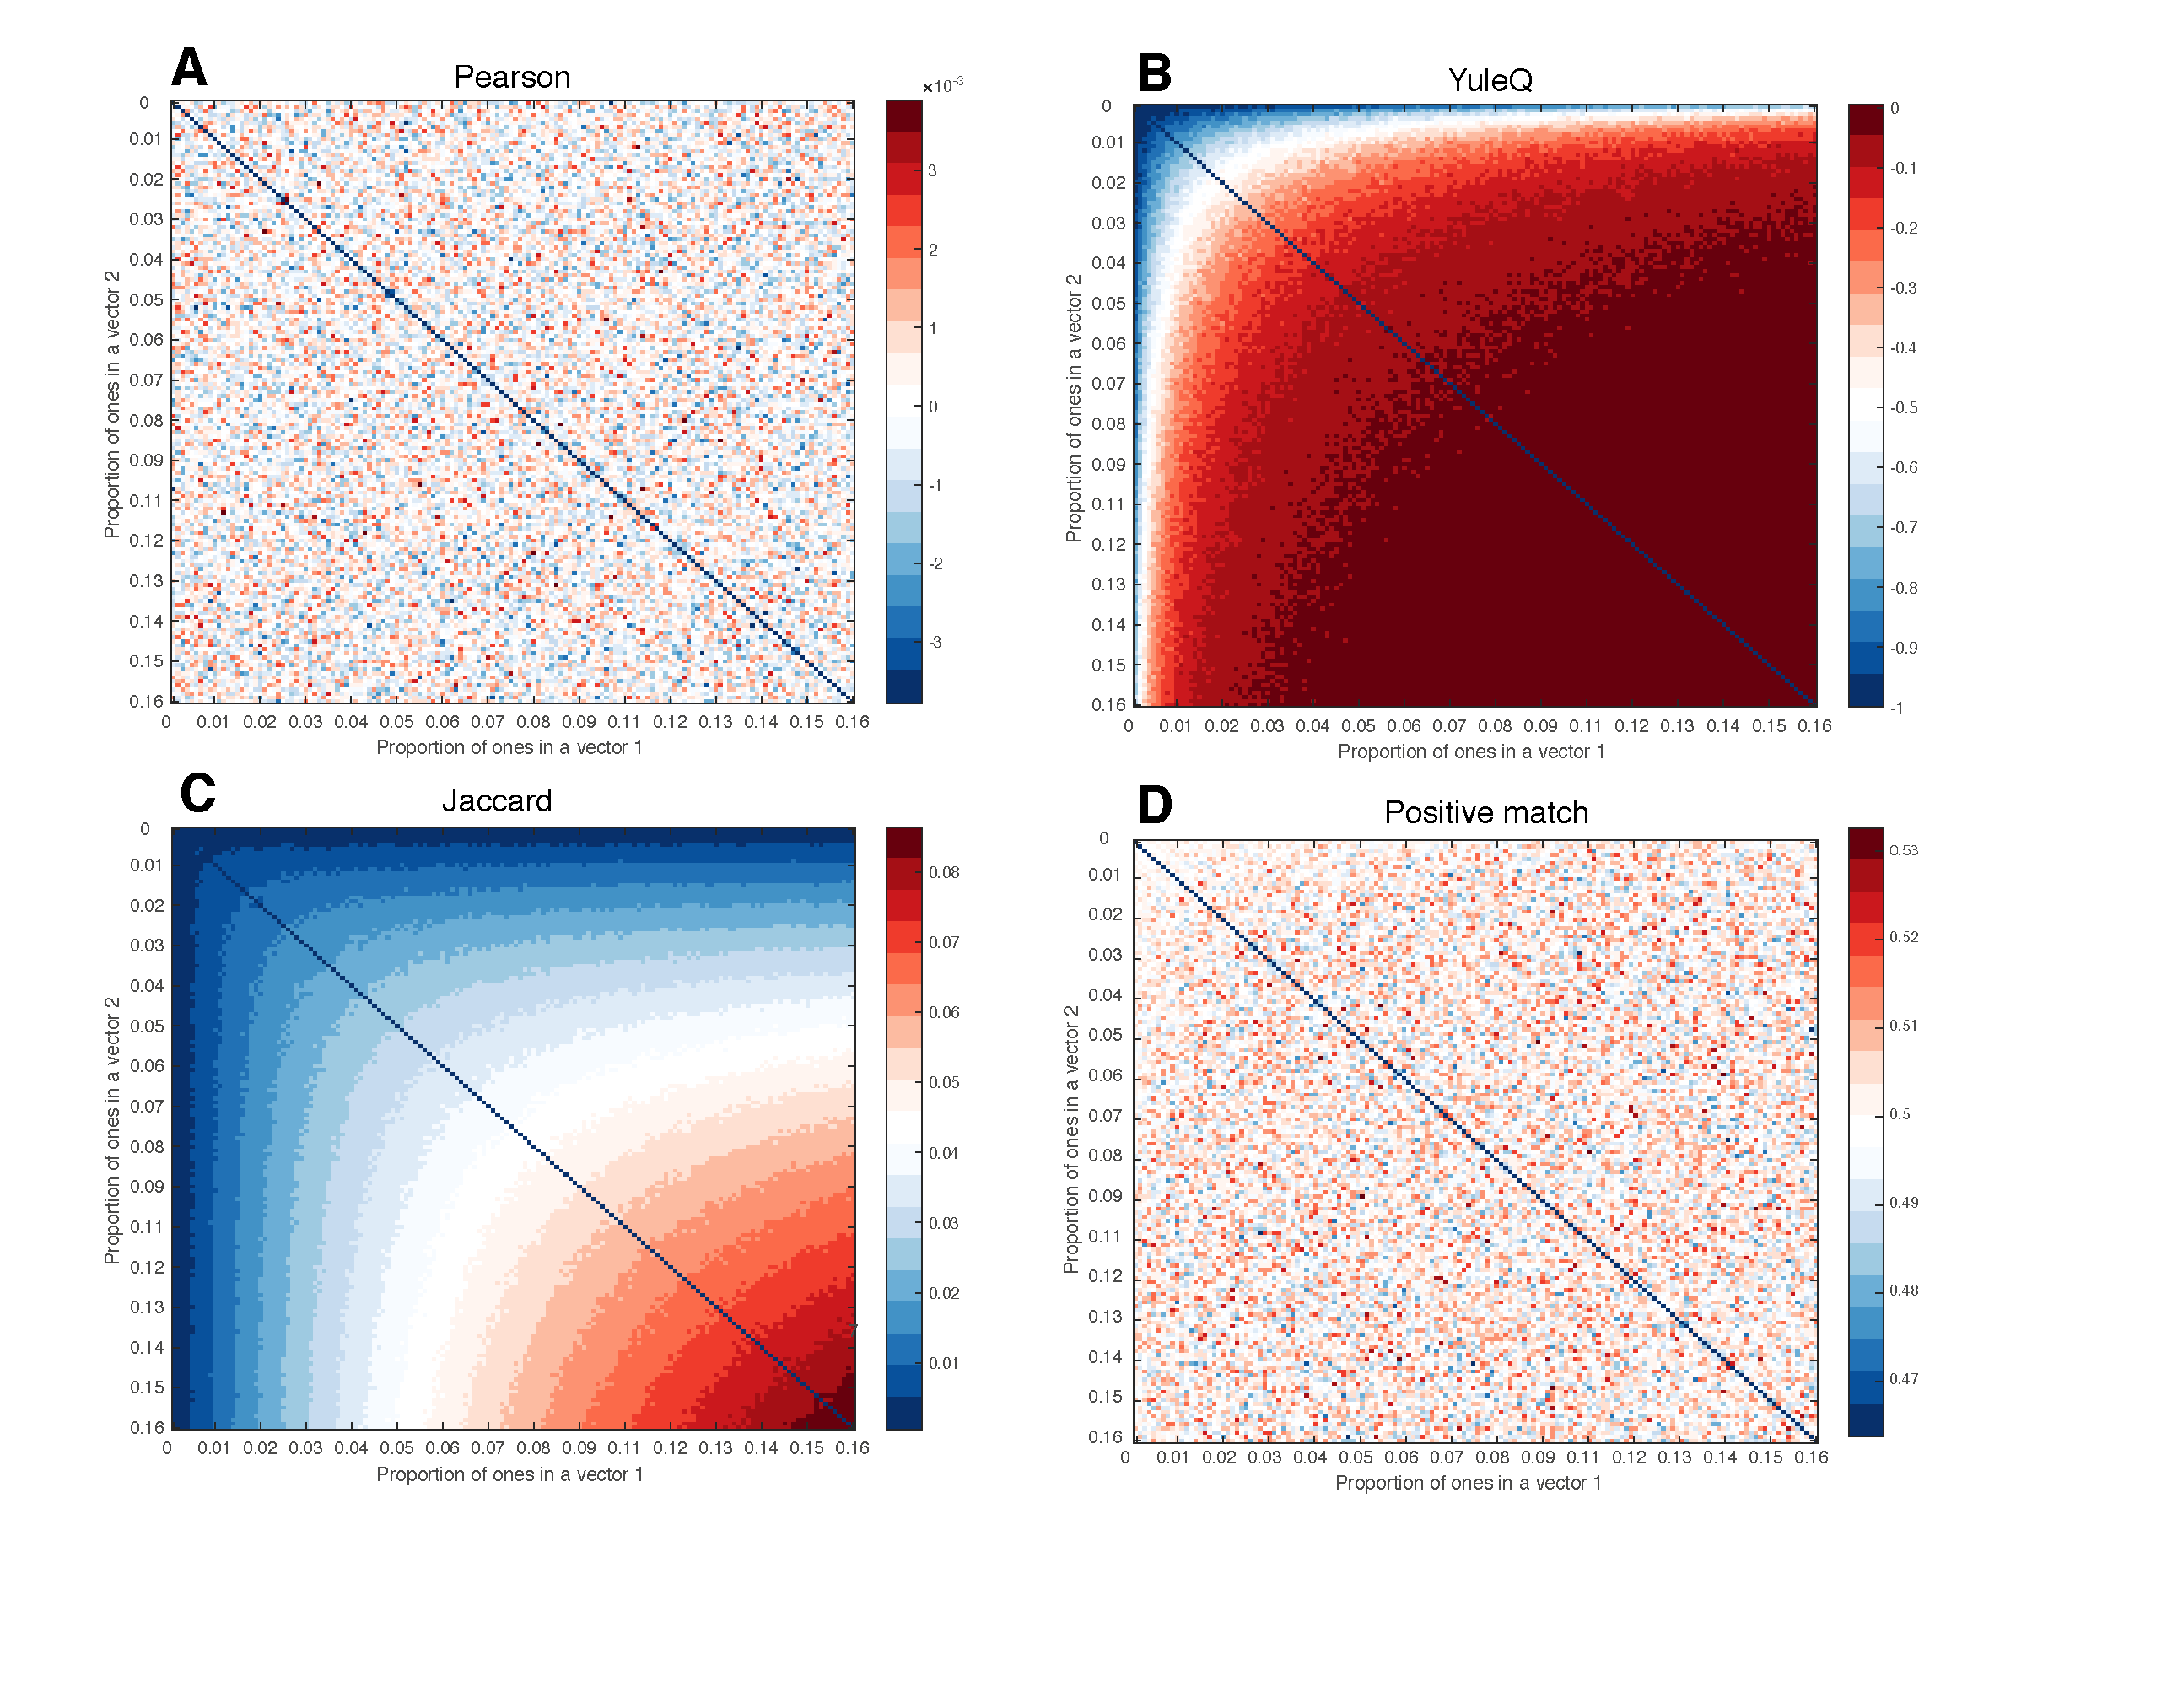
\includegraphics[width=1\textwidth]{CoexpressionMeasures.pdf}
\caption{
\textbf{Dependence of binary coexpression metrics to the proportion of positive annotations}
[[TODO: Add A, B, C labels, add our new positive match measure, provide better titles.]]
}
\end{figure}


\paragraph*{S2 Fig.}
{\bf Coexpression as a function of distance}

% <<runFigureGenerators>>: <<probabilityVSdistance, coexpressionDistance>>
\begin{figure}[h]
\centering
    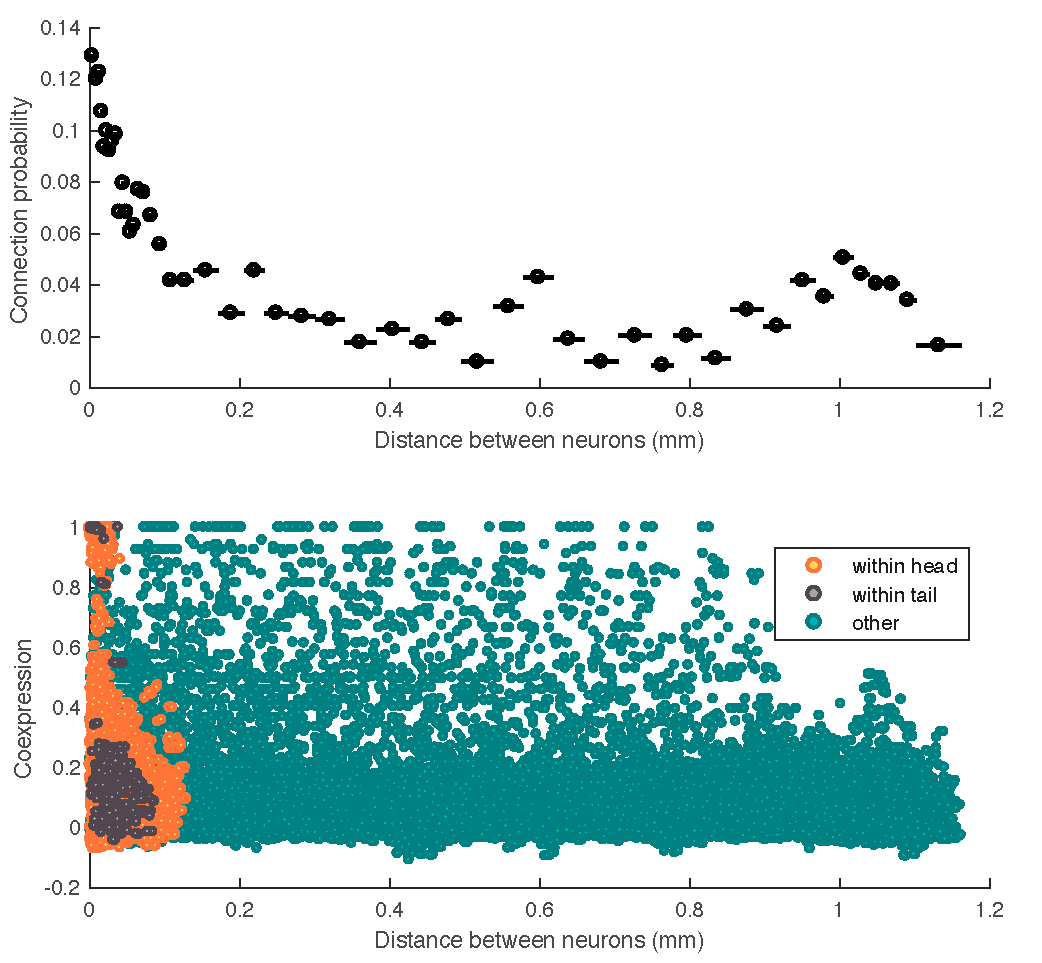
\includegraphics[width=1\textwidth]{distanceDependence.eps}
\caption{
\label{fig:S_distDep}
\textbf{Separation distance affects connection probability but not gene coexpression}
\textbf{A}
The connection probability is estimated in 50 equiprobable distance bins, shown as circles (bin centers) and lines (bin extent).
A decreasing relationship is evident up to a separation distance of approximately 0.2\,mm (driven by tail-tail and head-head connections), with a longer-range decrease up to $\approx$0.5\,mm due to body-body connections.
The increase at large distances ($\approx 1$\,mm) is due to head-tail connections, which also show a decay with distance, from $\approx 1$\,mm through to $\approx$1.2\,mm.
connections between body and head and body and tail showed no clear distance dependence.
[[should we show relationships by type here? It's in the Evernote: https://www.evernote.com/l/AF5h5EZ0dxZBU6RiKJk3BtNFs36tLrE4h0U]].
\textbf{B}
Pearson gene coexpression, $r_\phi$, is plotted as a function of separation distance for all pairs of neurons, labeled according to within-head (orange), within-tail (gray), and all other connections (aqua).
Unlike data from macroscopic mammalian brains of mouse \cite{Fulcher:2016ck} and human (\cite{Krienen:2016eq}), there is no clear spatial dependence in these neuronal data.
[[TODO: Did we check this is really true when we actually look across distance bins?]]
}
\end{figure}


% <<coexpRecUnidirUncon.m>>
\paragraph*{S3 Fig.}
{\bf Coexpression for rich, feeder and peripheral links as a function of degree.}
\begin{figure}[!h]
\label{S3_Fig}
\centering
    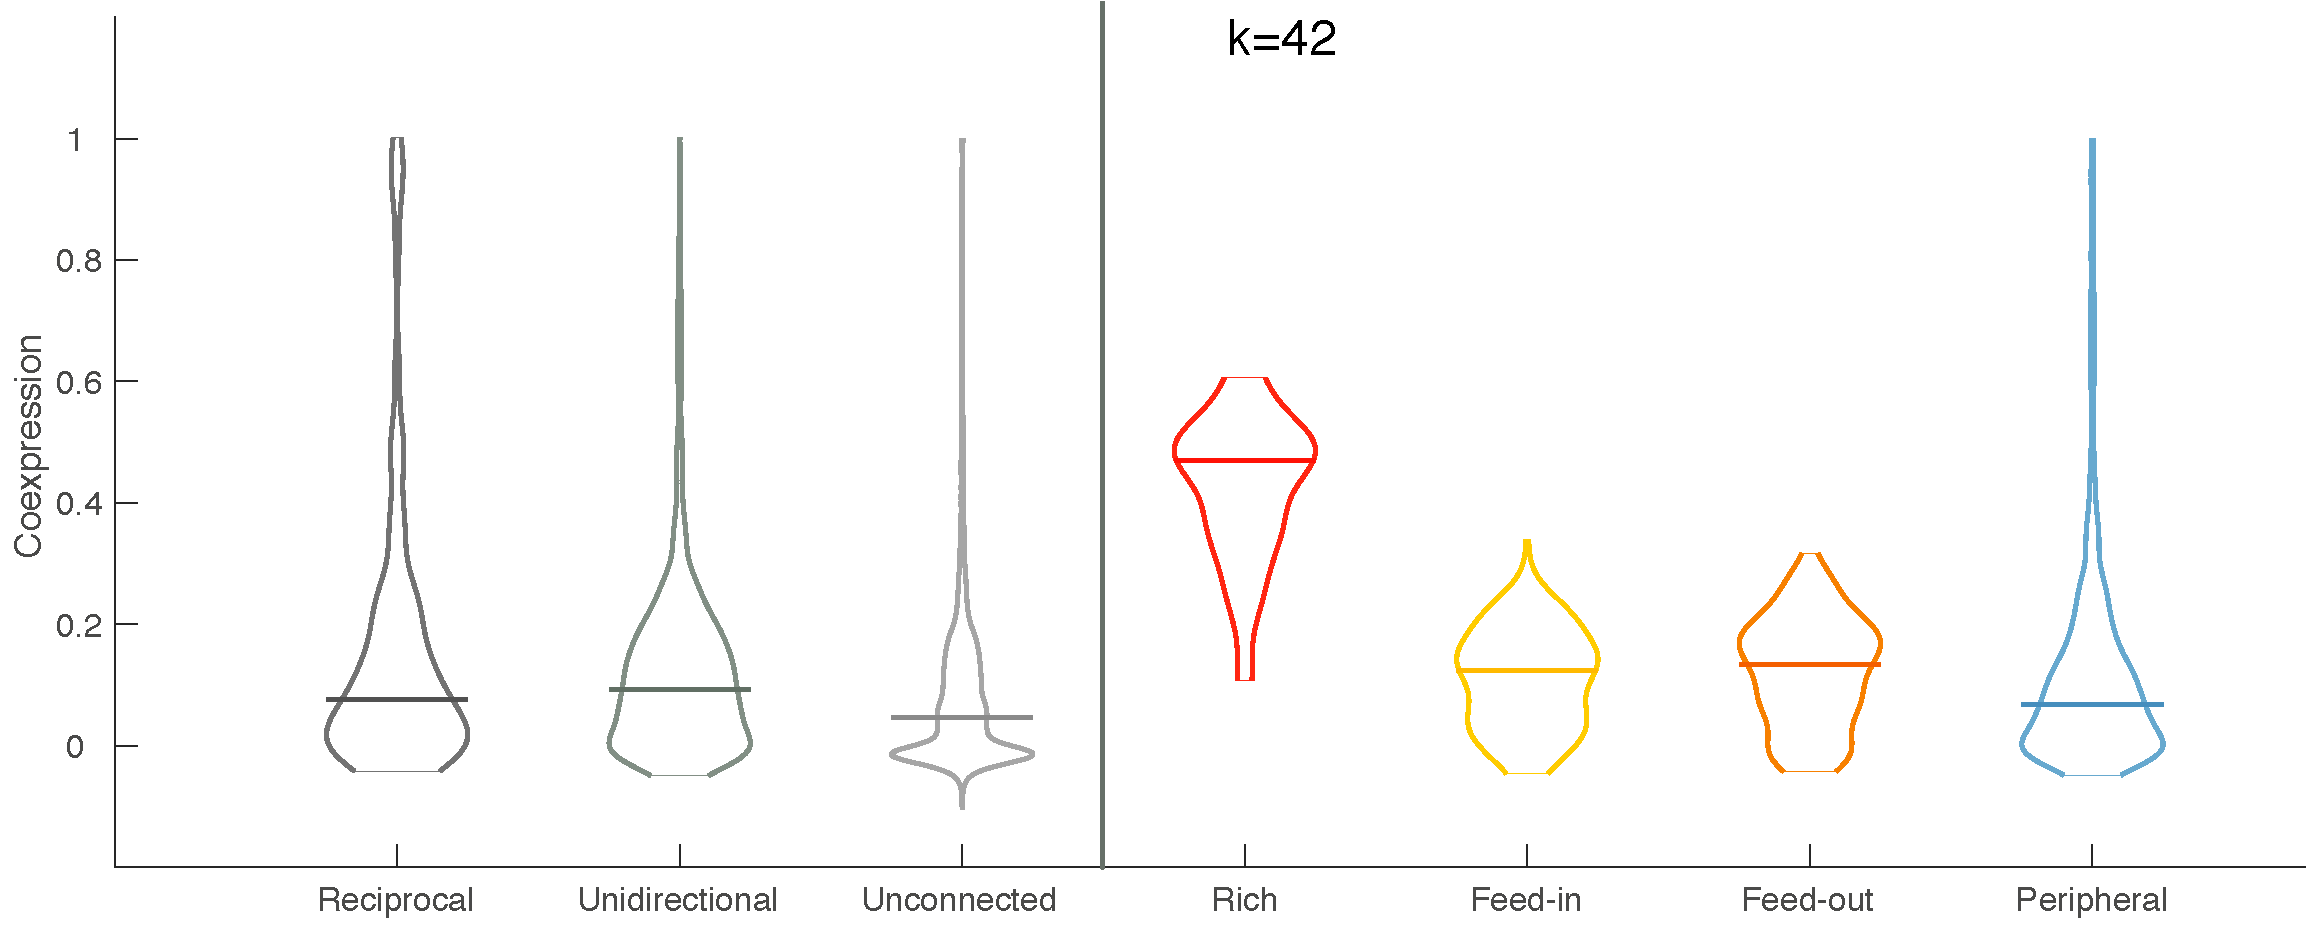
\includegraphics[width=1\textwidth]{Distributions.pdf}
\end{figure}

% <<networkRC.m>>
\paragraph*{S5 Fig.}
{\bf Weighted and mixed rich club}
\begin{figure}[!h]
\label{S5_Fig}
\centering
    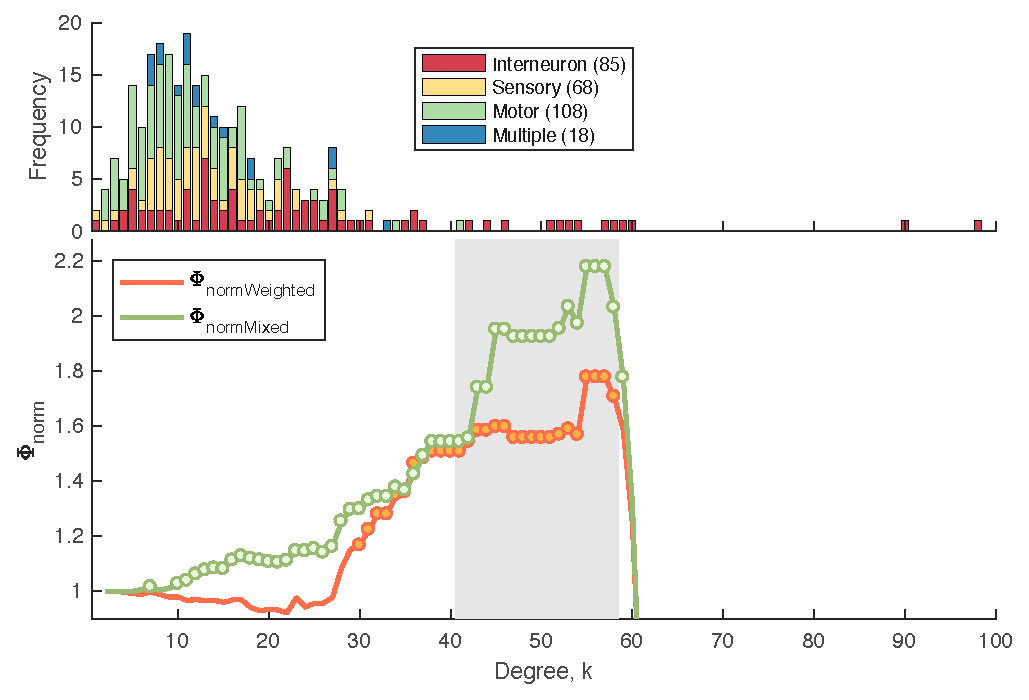
\includegraphics[width=1\textwidth]{WeightedMixedRC.pdf}
\end{figure}

% propTypesDegree(C) script
%\paragraph*{S6 Fig.}
%{\bf Neuron type and neurotransmitter as a function of degree}
%\begin{figure}[!h]
%\label{S7_Fig}
%\centering
%    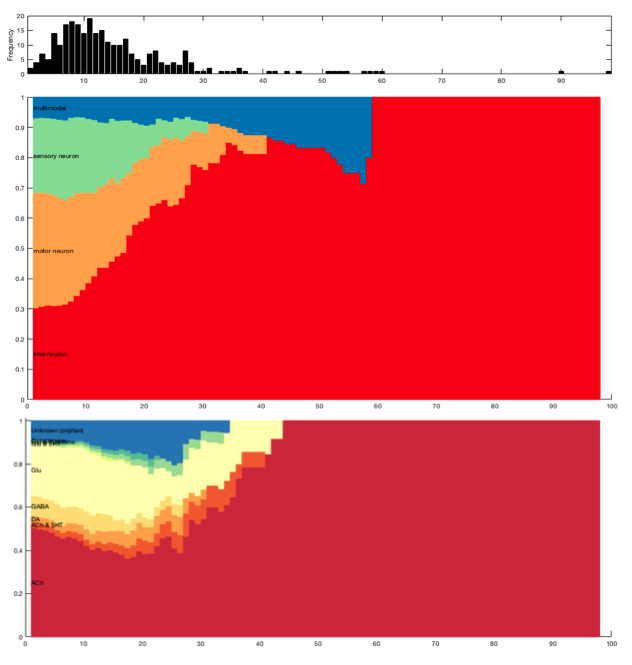
\includegraphics[width=0.7\textwidth]{TypeTransmitterDegree}
%\end{figure}

% RichClub script
\paragraph*{S7 Fig.}
{\bf Average coexpression for rich, feeder and peripheral links as a function of degree.}
Top: degree distribution. Average gene coexpression for rich, feeder, and peripheral connections as a function of \textit{k}, with the mean across all network links shown as a dashed black line and the topological rich club regime shaded grey.
Circles indicate a statistically significant increase in gene coexpression in a given link type relative to the rest of the network (one-sided Welch’s t-test; $P < 0.05$)
\begin{figure}[!h]
\label{S7_Fig}
\centering
    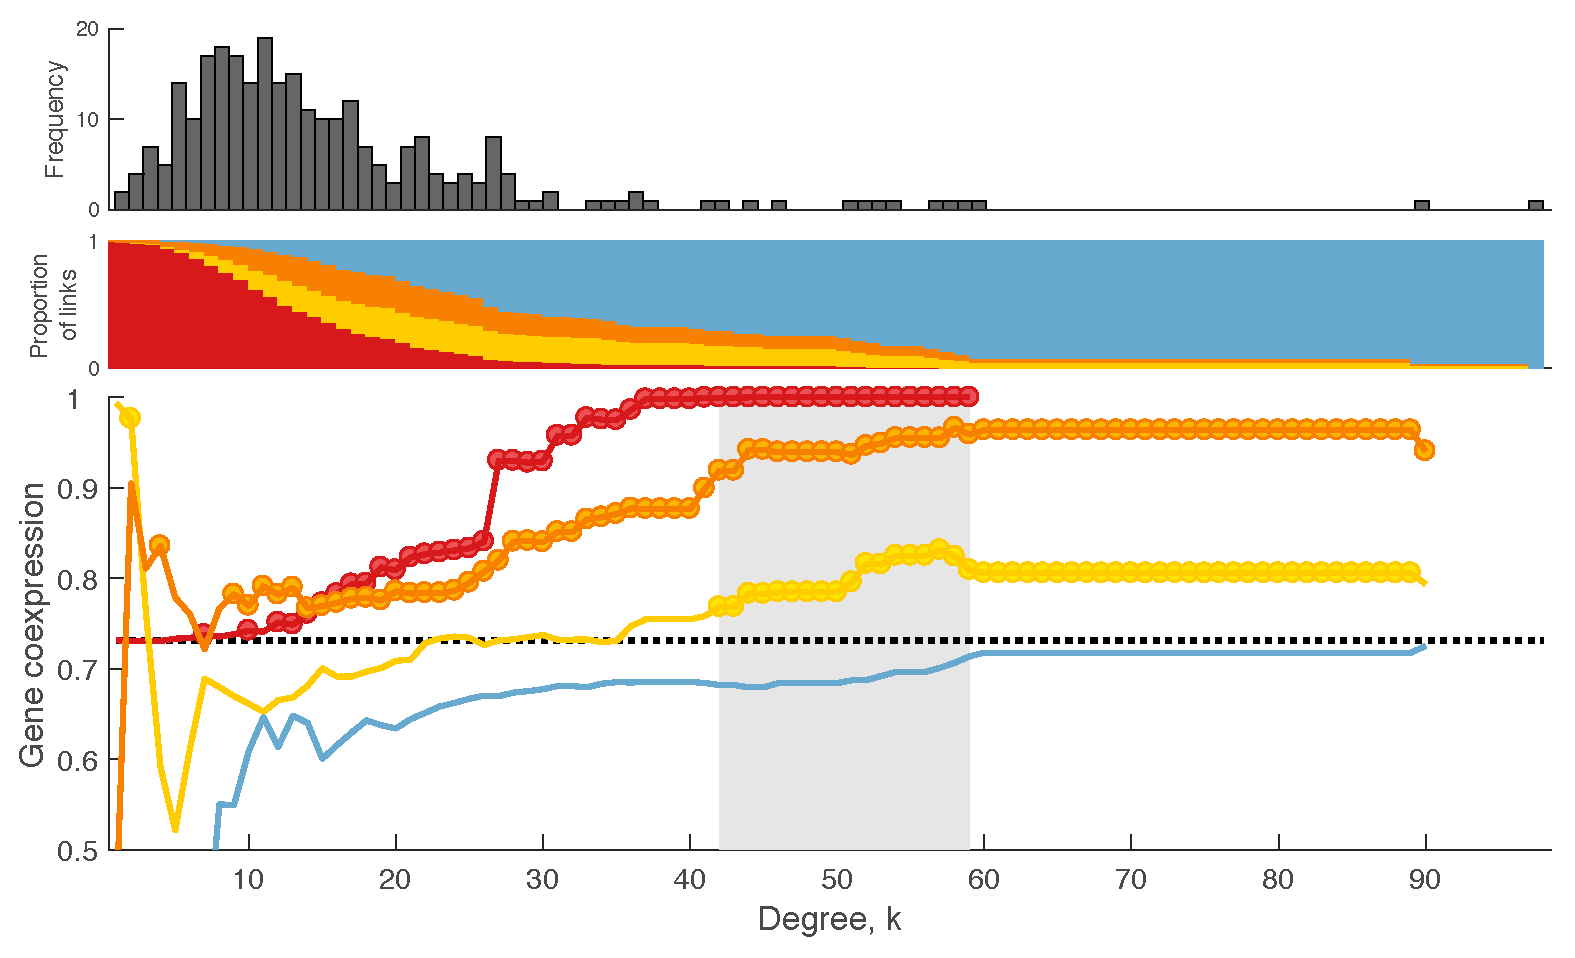
\includegraphics[width=1\textwidth]{coXmeanCoexpression.pdf}
\end{figure}




\end{document}
